%%%%%%%%%%%%%%%%%%%%%%%%%%%%%%%%%%%%%%%%%%%%%%%%%%%%%%%%%%%%%%%%%%%%%%%%%%%%%%%%
%%%%%%%%%%%%%%%%%%   Vorlage für eine Abschlussarbeit   %%%%%%%%%%%%%%%%%%%%%%%%
%%%%%%%%%%%%%%%%%%%%%%%%%%%%%%%%%%%%%%%%%%%%%%%%%%%%%%%%%%%%%%%%%%%%%%%%%%%%%%%%

% Erstellt von Maximilian Nöthe, <maximilian.noethe@tu-dortmund.de>
% ausgelegt für lualatex und Biblatex mit biber

% Kompilieren mit
% latexmk --lualatex --output-directory=build thesis.tex
% oder einfach mit:
% make

\documentclass[
  tucolor,       % remove for less green,
  BCOR=12mm,     % 12mm binding corrections, adjust to fit your binding
  parskip=half,  % new paragraphs start with half line vertical space
  open=any,      % chapters start on both odd and even pages
  cleardoublepage=plain,  % no header/footer on blank pages
]{tudothesis}


% Warning, if another latex run is needed
\usepackage[aux]{rerunfilecheck}

% just list chapters and sections in the toc, not subsections or smaller
\setcounter{tocdepth}{1}

%------------------------------------------------------------------------------
%------------------------------ Fonts, Unicode, Language ----------------------
%------------------------------------------------------------------------------
\usepackage{fontspec}
\defaultfontfeatures{Ligatures=TeX}  % -- becomes en-dash etc.

% german language
\usepackage{polyglossia}
\setdefaultlanguage{german}

% for english abstract and english titles in the toc
\setotherlanguages{english}

% intelligent quotation marks, language and nesting sensitive
\usepackage[autostyle]{csquotes}

% microtypographical features, makes the text look nicer on the small scale
\usepackage{microtype}

%------------------------------------------------------------------------------
%------------------------ Math Packages and settings --------------------------
%------------------------------------------------------------------------------

\usepackage{amsmath}
\usepackage{amssymb}
\usepackage{mathtools}
\usepackage{bbold}

% Enable Unicode-Math and follow the ISO-Standards for typesetting math
\usepackage[
  math-style=ISO,
  bold-style=ISO,
  sans-style=italic,
  nabla=upright,
  partial=upright,
]{unicode-math}
\setmathfont{Latin Modern Math}

% nice, small fracs for the text with \sfrac{}{}
\usepackage{xfrac}


%------------------------------------------------------------------------------
%---------------------------- Numbers and Units -------------------------------
%------------------------------------------------------------------------------

\usepackage[
  locale=DE,
  separate-uncertainty=true,
  per-mode=symbol-or-fraction,
]{siunitx}
\sisetup{math-micro=\text{µ},text-micro=µ}
% \sisetup{tophrase={{ to }}}
%------------------------------------------------------------------------------
%-------------------------------- tables  -------------------------------------
%------------------------------------------------------------------------------

\usepackage{booktabs}       % \toprule, \midrule, \bottomrule, etc

%------------------------------------------------------------------------------
%-------------------------------- graphics -------------------------------------
%------------------------------------------------------------------------------

\usepackage{graphicx}
%\usepackage{rotating}
\usepackage{grffile}
\usepackage{tikz}
\usepackage{circuitikz}
\usepackage{tikz-feynman}
\usepackage{subcaption}

% allow figures to be placed in the running text by default:
\usepackage{scrhack}
\usepackage{float}
\floatplacement{figure}{htbp}
\floatplacement{table}{htbp}

% keep figures and tables in the section
\usepackage[section, below]{placeins}


%------------------------------------------------------------------------------
%---------------------- customize list environments ---------------------------
%------------------------------------------------------------------------------

\usepackage{enumitem}
\usepackage{listings}
%------------------------------------------------------------------------------
%------------------------------ Bibliographie ---------------------------------
%------------------------------------------------------------------------------

\usepackage[
  backend=biber,   % use modern biber backend
  autolang=hyphen, % load hyphenation rules for if language of bibentry is not
                   % german, has to be loaded with \setotherlanguages
                   % in the references.bib use langid={en} for english sources
]{biblatex}
\addbibresource{references.bib}  % the bib file to use
\DefineBibliographyStrings{german}{andothers = {{et\,al\adddot}}}  % replace u.a. with et al.


% Last packages, do not change order or insert new packages after these ones
\usepackage[pdfusetitle, unicode, linkbordercolor=tugreen]{hyperref}
\usepackage{bookmark}
\usepackage[shortcuts]{extdash}

%------------------------------------------------------------------------------
%-------------------------    Angaben zur Arbeit   ----------------------------
%------------------------------------------------------------------------------

\author{Nils Breer}
\title{Alignment studies for the LHCb SciFi Detector}
\date{2022}
\birthplace{Unna}
\chair{Lehrstuhl für Experimentelle Physik IV}
\division{Fakultät Physik}
\thesisclass{Master of Science}
\submissiondate{May 4th 2022}
\firstcorrector{Prof.~Dr.~Albrecht}
\secondcorrector{Prof.~Dr.~Weingarten}

% tu logo on top of the titlepage
\titlehead{
\includegraphics[height=1.5cm]{logos/tu-logo.pdf}}

\begin{document}
\frontmatter
\maketitle

% Gutachterseite
\makecorrectorpage

% hier beginnt der Vorspann, nummeriert in römischen Zahlen
\chapter*{Abstract}
\label{sec:abstract}

% general analysis of the scifi detector regarding alignment
% what i have done and how alignment in general has worked out
% difficulties?

% In dieser Bachelorarbeit wird ein Algorithmus zur Rekonstruktion
% von Λ-Baryonen implementiert, welcher auf bereits bestehenden
% Algorithmen zur Rekonstruktion von Kaonen aufbaut und zur Verbesserung
% von Strange-Tagging beiträgt.
% Strange-Tagging ist eine Form des Flavortaggings, welche darauf
% ausgelegt ist, Hadronen mit Strange-Quarks zu identifizieren.
% Vor allem f\"ur neutral geladene Hadronen, welche mindestens ein
% Strange-Quark als Parton tragen ist es interessant
% herauszufinden in welchen Prozessen diese entstehen.
% Au\ss erdem kann das Strange-Tagging dabei helfen, neue Erkenntnisse
% \"uber das CKM-Matrix Element $|\symup{V}_{ts}|$ zu erzielen.
% Dafür werden verschiedene Objekte herangezogen, welche zwischen
% Strange-Quark-Jets und Up-Quark-Jets beziehungsweise Down-Quark-Jets
% diskriminieren.
% Es ergibt sich, dass die Objekte $X_{\symup{\Lambda}}$ und
% $\symup{\Delta R}$ gut zwischen Strange-Jets von Down- und Up-Jets
% diskriminieren doch die Masse des $\symup{\Lambda}$-Baryons daf\"ur
% nicht geeignet ist.

\chapter*{Kurzfassung}
\label{sec:kurzf}

% general analysis of the scifi detector regarding alignment
% what i have done and how alignment in general has worked out
% difficulties?

Hier steht das selbe wie im Abstract nur auf deutsch.

\tableofcontents

\mainmatter
% Hier beginnt der Inhalt mit Seite 1 in arabischen Ziffern
\chapter{Introduction}
\label{sec:einleitung}

At the beginning of the $20^{\text{th}}$ century many physicists started research on
elementary particles and the interactions associated with them. The combined
knowledge lead to the construction of one of the most precisely tested theories: the Standard Model (SM) of particle physics.
Flavour anomalies show strong tensions with the Standard Model and also the recent publication on the W-boson mass measurement is challenging the accuracy of the Standard Model\cite{wmass}.
No single measurement or anomaly on its own is enough to be in a total disagreement with the SM, but combined they provide hints that the SM is not the final theory.
The SM describes every fundamental force except for gravity. There are still open questions such the baryon asymmetry of the universe requiring a, by several orders of magnitude, larger charge-parity (CP) violation than the SM predicted.
To tackle these problems, high energy experiments such as the Large Hadron Collider beauty (LHCb) experiment located at the Large Hadron Collider (LHC) at CERN were built for this exact reason.
The LHCb experiment was designed to study beauty and charm quarks with focus on measuring CP-violation and searching for New Physics in rare decays.
To detect these phenomena, the threshold for statistical uncertainties has to
be lowered and the amount of data collected needs to be increased. The LHCb upgrade described in section \ref{sec:upgradeLHCb} allows us to have a five times higher instantaneous luminosity of $\SI{2e33}{\invfb}$ with the expected detector readout rate of $\SI{40}{\mega\hertz}$.
To realize these hardware and software challenges, the front-end electronics, tracking systems and the trigger system needed upgrades.
The tracking system has been replaced with a single tracker based on scintillating fibres that is currently commissioned. The physics performance is highly dependent on how well the detector is aligned, since poor alignment leads to systematic biases which can have a negative impact on sensitive asymmetry measurements. It can also lead to worse mass resolution. Therefore it is crucial that the SciFi detector is well aligned.
To operate the upgraded LHCb at its full potential, it is of great importance that all detector components are brought into an alignment level so that the impact on physical observables is insignificant.
\\
\\
The Alignment theory will be described in chapter \ref{sec:alignTheory}. In chapter \ref{sec:story} different sets of constraints, degrees of freedom
and alignable objects called \textit{configuration} will be tested first in order
to study how different configurations influence the alignment. Afterwards several
tests will be performed to analyse the behavior of a misaligned detector and check
if the chosen configuration converges towards an aligned state.
The deviations from a centered state after the alignment are needed for other trigger stages to be known in the reconstruction.
The LHC will not run permanently at maximum luminosity therefore tests are performed to analyse alignment of different luminosity samples. Especially while the LHC restarts it will run at a lower luminosity.
During the alignment studies a bias inside the Scintillating Fibre hit clustering algorithms was discovered which had an impact on the alignment. The exact changes will be discussed in the final section of chapter \ref{sec:story}.

% finished

% theory
\chapter{Particles and The Large Hadron Collider}
\label{sec:particleslhc}

With good alignment, studies on all Standard Model particles and hadron states
will improve. Yielding better efficiencies on SM particle measurements will
result in deeper insights regarding physics beyond the stand modell from high-precision measurements of CP-violating observables as an example.

On a grand scheme upgrading the LHCb and therefore the LHC will bring deeper
insights "for" (wrong word) standard model processes. To understand the universe even better and eventually yield information about the unsolved question of "dark matter" and
"dark energy", what is believed to be the bulk of the universes content.

\section{The Standard Model}
\label{sec:sm}

\begin{figure}
  \centering
  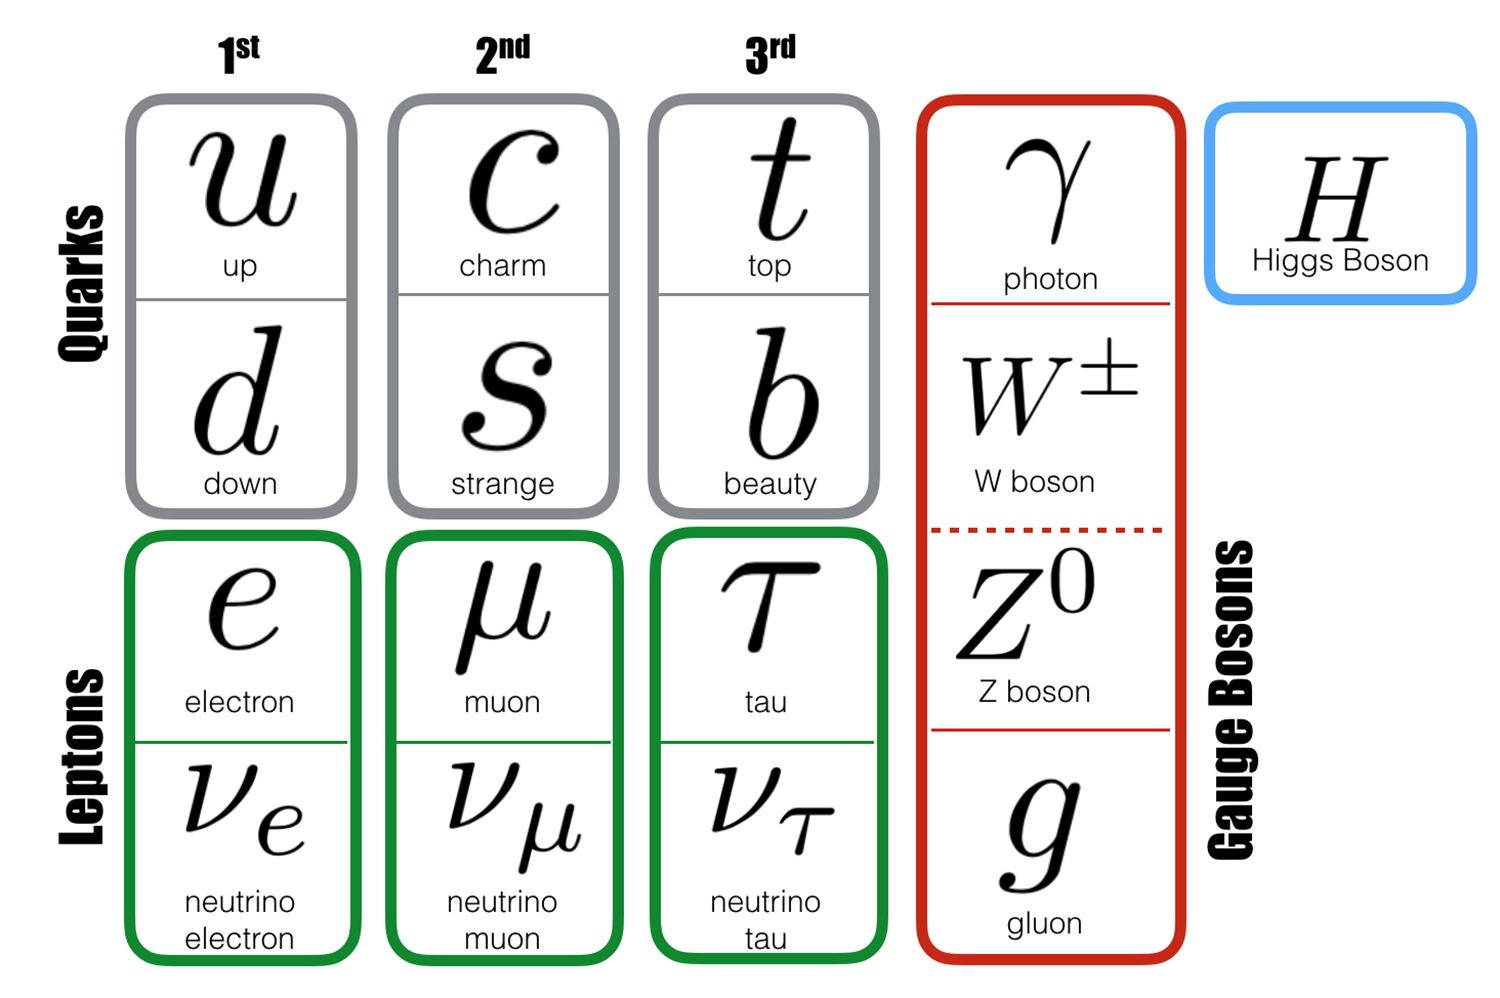
\includegraphics[width=0.75\textwidth]{plots/SM_2018.png}
  \caption{The standard model of particle physics\cite{standard2018}.}
  \label{fig:sm2018}
\end{figure}

The standard model of particle physics\ref{fig:sm2018} describes the known elementary particles and their interactions. It consists of 12 matter particles, the fermions
and five interaction particles, which are called vector bosons.

The fermions 12 spin-$\frac{1}{2}$ particles. Six are called leptons and they are sorted into three families, also called flavors (e, $\mu$ and $\tau$) and six are called quarks. Each of those lepton families has a charged lepton\footnote{can have both h\"ndigkeiten} and a left-handed neutrino.
A particle is called left-handed if its spin direction is opposite to the direction of flight. Right-handed particles have a spin direction pointing with the direction of flight.
Neutrinos can only be left-handed since there is no system where the neutrino can be "overtaken" so the momentum switches and therefore the helicity.
A left-handed isospin doublet and a left-handed singlet can be constructed.
The leptons can couple via the weak-interaction and if they are charged, also via the em-interaction. Neutrinos can only couple via the weak interaction.
Each matter particle also has an antiparticle, with an opposite charge.

The quarks are spin-$\frac{1}{2}$-fermions and carry an electric charge as well. In each of the three generations there is one isospin doublet. The quarks are ordered by ascending mass. In the first generation are the two lightest quarks,
up- and down quark, in the second generation the charm- and strange quark and
in the third generation the top- and bottom quark doublet.
Quarks carry a color charge, red, green or blue, which is an artificially introduced degree of freedom to guarantee the distinguishability.

%---------- interactions -----------
The interactions are obtained from the vector bosons mentioned above.
The three potent interactions are the electromagnetic(em) interaction,
the weak interaction and the strong interaction. Gravitation does not make a significant contribution.
The vector boson of the em interaction is the photon which is exchanged between particles.
% here, a feynman diagram would be nice. as well as for every other force
The strength of one of those interactions is
described by a coupling constant. In the em interaction this is the
fine structure constant\cite{alphas}. The range of the em-interaction is in principle
infinite, but decreases with increasing distance between the interacting particles.
The em interaction is described by quantum electrodynamics.
The potentials are described by operators, which create and annihilate the photons.

The exchange particles of the weak interaction are on the one hand the $W^{\pm}$-bosons and on the other hand the Z-boson.
The weak interaction processes are called currents.
Changing the charge during the interaction by a W-boson is called charged current.
The exchange reaction of a Z boson in, for example, processes such as $e_{\nu} \mu \to e_{\nu} \mu$ is called neutral current.
Analogous to the electromagnetic interaction, the potentials are again understood as
operators, but here there are no propagators. Propagators are
used in \textit{FEYNMAN}-diagrams of QED to represent the interaction particles.
A so-called V-A structure is used here instead. Here, V stands for vectorboson and A is the axialvector.
This structure is needed to disregard the right-handed particles and left-handed
antiparticles, since these lead to the charge-parity violation. Thus the Lorentz factors are adjusted in the following way
\begin{equation*}
  \gamma_{\mu} \to \gamma_{\mu}(1 - \gamma_5)
\end{equation*}
Quarks couple via the strong interaction which is described by the quantum chromodynamic (QCD). The Eichgroup of the QCD is $SU\left(N = 3\right)$ where N is the number of introduced colors as a new degree of freedom. The number of generators is therefore $N^2 - 1 = 8$.
The generators are called gluons and they carry color and anticolor, have no mass and carry spin 1.
Gluons can, other than photons, couple to themselves.
Moreover, the coupling constant $\alpha_s \approx 0.1$. The interaction with quarks is described with a potential.
\begin{align}
  \symup{V}_{q\bar{q}} &= -\frac{4 \alpha_{s}}{3 r} + \sigma\cdot r
  \intertext{with}
  \sigma &= \SI{1}{\giga\electronvolt\per\femto\metre}
\end{align}
The common eight gluon-wavefunctions\cite{qcd} are
\begin{align*}
  \psi_1 &= |r\bar{g}> & \psi_2 &= |r\bar{b}> \\
  \psi_3 &= |g\bar{r}> & \psi_4 &= |g\bar{b}> \\
  \psi_5 &= |b\bar{r}> & \psi_6 &= |b\bar{g}> \\
  \psi_7 &= \frac{1}{\sqrt{2}}\left(|r\bar{r}> - |g\bar{g}>\right) & \psi_8 &= \frac{1}{\sqrt{6}}\left(|r\bar{r}> + |g\bar{g}> - 2|b\bar{b}>\right) \\
\end{align*}

The second wavefunction describes a gluon interaction with a blue quark and changing the color to red.

Quarks thus tend to attract each other very strongly. If now
quark and anti quark are moved away from each other, a lot of energy has to be expended. This energy can become so large that new particles can be created.

Due to the Confinement, quarks cannot exist alone. Instead they form bonding states, so called hadrons. On the one hand there are the mesons, which consist of a quark
and an antiquark.

\begin{equation}
	|\symup{M}\!> = | q\, \bar{q}'\!>
\end{equation}

These may be from the same family (i.e. [u,d], [c,s], [t,b]), or from
different families. Mesons have a baryon number of 0. Accordingly, quarks carry the baryon number $\frac{1}{3}$. The quarks constructing a meson therefore carries color and the corresponding anticolor.
The second type are baryons. The content consists of either three quarks or
three antiquarks. However, it cannot be that one quark and two antiquarks
and vice versa occur, because baryons must have the baryon number $\symup{B} = 1$. Because baryons are stable final states as well as the mesons, the sum of their quark colors must be white. Therefore, every (anti)color must occur once in a baryon.

\begin{align}
	|\symup{B}\!> &= |q q' q''\!> \\
	|\symup{\bar{B}}\!> &= |\bar{q} \bar{q}' \bar{q}''\!> \,
\end{align}

\section{particle decays and hadrons}
\label{sec:decays}

\section{The LHC and LHCb}
\label{sec:lhcandB}

\subsection{The LHC}
The Large Hadron Collider (LHC)\cite{lhcInfo} is the most powerfull particle-accelerator on planet earth. With a circumference of $26,7\si{\kilo\metre}$ it is also the longest ring accelerator and it lies between $45\si{\metre}$ and $170\si{\metre}$ below the surface near Geneva in Swizerland. The tunnel was constructed for the LEP experiment between 1984 and 1989 and is operated by the European Organization for Nuclear Research (CERN). The LHC can produce centre of mass energies of $\sqrt{s} = \SI{13}{\tera\electronvolt}$ in proton-proton collisions during Run 2. After the upgrade the LHC will collide particles with the centre of mass energy of around $\sqrt{s} = \SI{14}{\tera\electronvolt}$.
An image of the accelerators and the experiments is shown in fig. \ref{fig:CERN}.

\begin{figure}
  \centering
  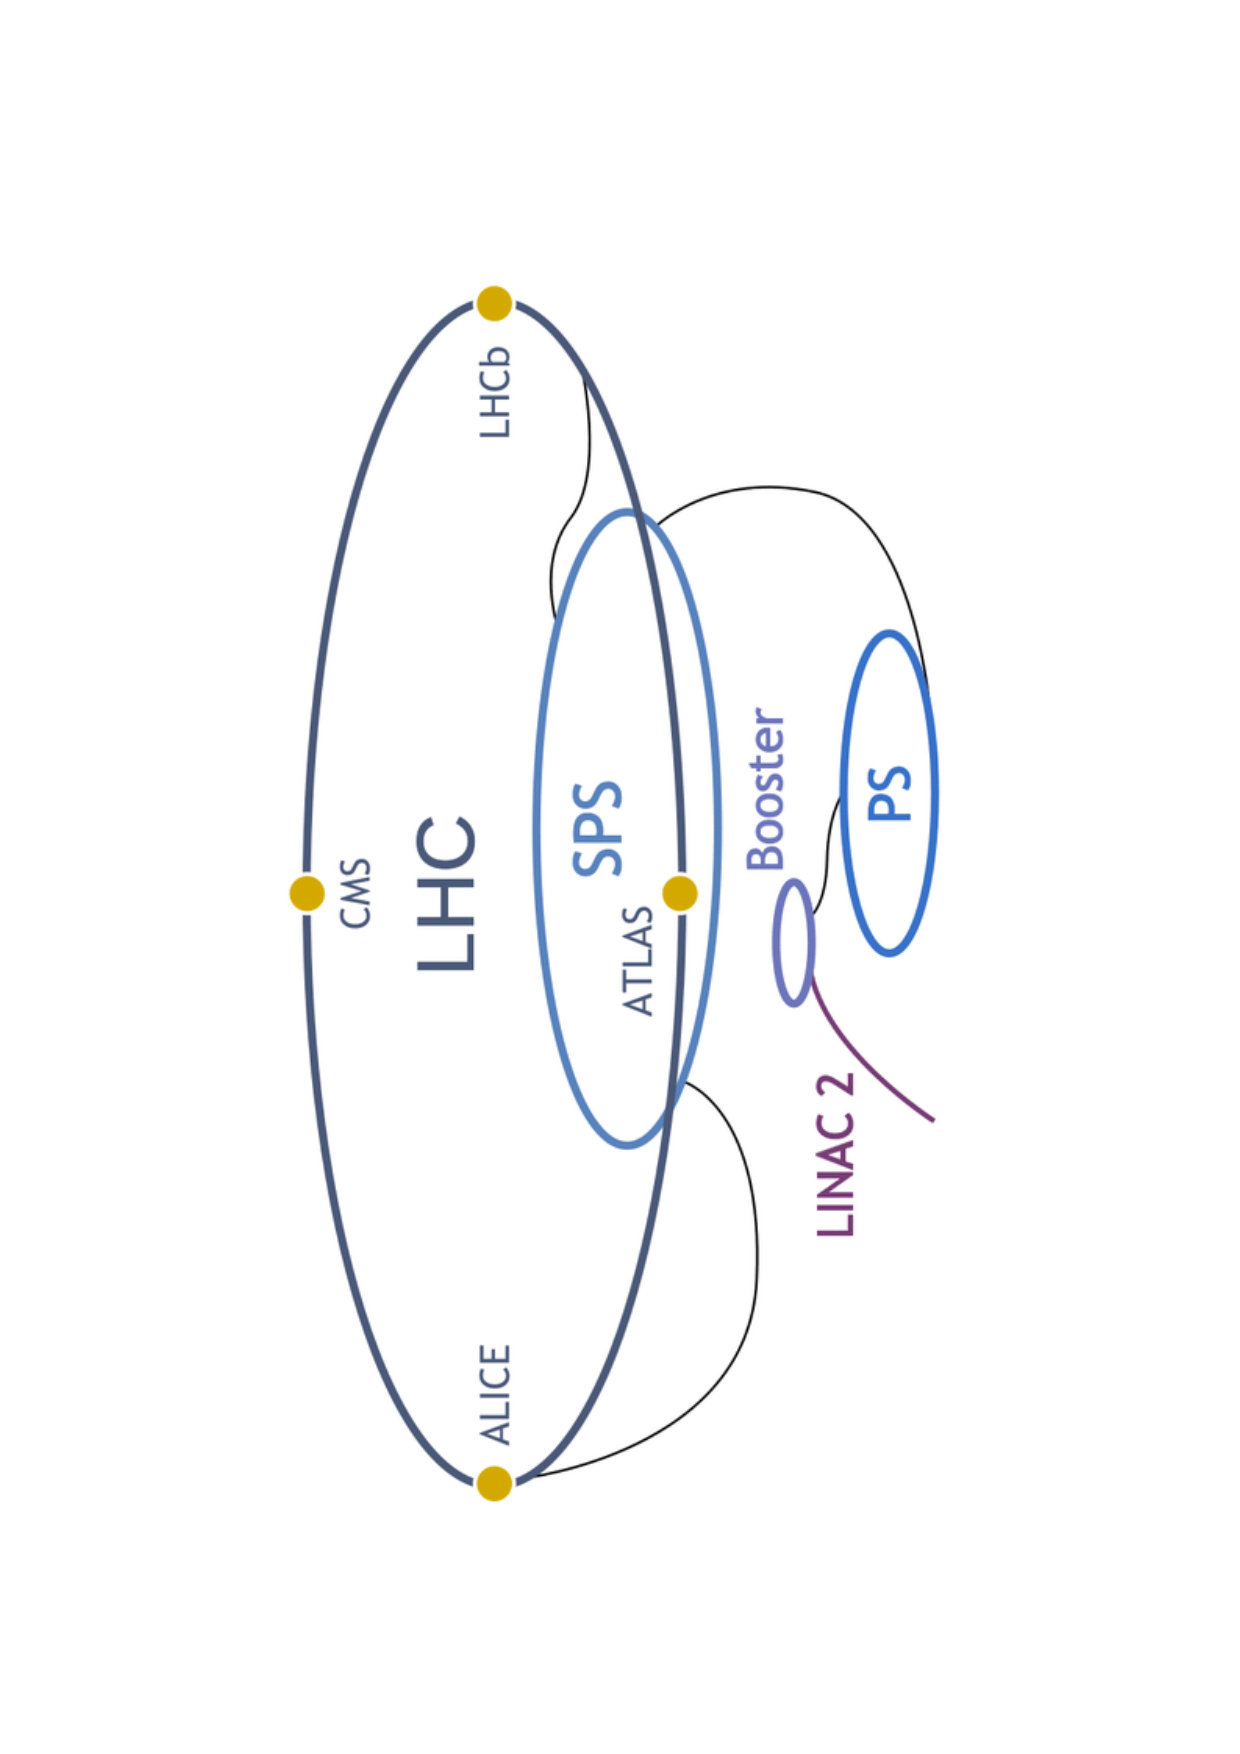
\includegraphics[angle=-90, origin=c, width=0.7\textwidth]{plots/CERN_layout.pdf}
  \caption{an overview of the LHC facilities\cite{facilityCERN}.}
  \label{fig:CERN}
\end{figure}

By ionizing hydrogen gas, protons are created and accelerated to $\SI{50}{\mega\electronvolt}$ by the linear accelerator (LINAC 2). Afterwards the beam is injected into the Proton Syncrotron and the Super Proton Synchrotron to a maximum of $\SI{450}{\giga\electronvolt}$ before the beam is brought into the LHC.
The beam containts several bunches with around $\num{1.15e11}$ protons per bunch and a bunch spacing of $\SI{25}{\nano\second}$.%., which is a collision rate of $\SI{40}{\mega\hertz}$.
The LHC houses four major experiments. ATLAS and CMS are classified as general purpose detectors with a detection range of close to $4\pi$. The interaction in these detectors is located in the very center so that tracks going in every direction can possibly be found. Searches for the Higgs Boson is just one of many physics aspects these detectors are build for.
The other two Experiments located at the LHC are ALICE and LHCb.
The ALICE experiment mainly studies the quark-gluon plasma during the runs with lead ion collisions instead of protons.
In this thesis the Scintillating Fibre Tracker (SciFi Tracker) located at the LHCb will be focused at and discussed on the following chapters.

\subsection{The LHCb}
\label{sec:upgradeLHCb}

\begin{figure}
  \centering
  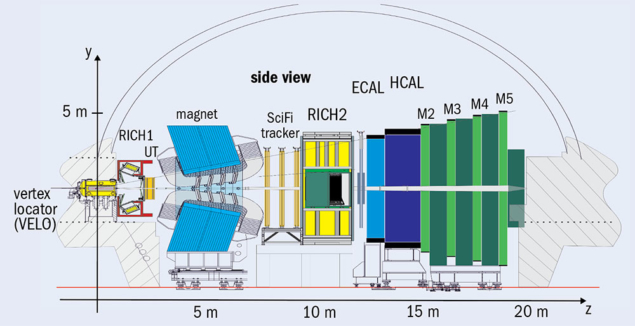
\includegraphics[width=0.75\textwidth]{plots/LHCb_facility.jpg}
  \caption{a sideview of the LHCb experiment\cite{facilityLHCb}.}
  \label{fig:LHCb}
\end{figure}

For high energies, b- and $\bar{b}$-hadrons are heavily produced in a tight forward
direction\ref{fig:bbforward}\footnote{They are also produced in a tight backward
direction but the experiment is only build for the forward cone.}.
The LHCb experiment\cite{lhcbInfo} is a forward spectrometer covering
$2 \,<\, \eta \,<\, 5$ in the pseudorapidity range. This experiments main
physics goal is beauty quark physics. A sideview of
the LHCb is shown in figure \ref{fig:LHCb}.
The LHCb consists of several smaller detector components namely the Vertex Locator
(VELO) right on the intercation point, two Ring Imaging Cherenkov counter
(RICH 1 and RICH 2), in front of the spectrometers lies the Trigger Tracker and
behind them the SciFi Tracker which is the important part of this thesis. Further
back a Preshower (PS) is mounted followed
by the electromagnetic calorimeter (ECAL) and the hadronic calorimeter (HCAL).
In the very back, several muon chambers are mounted for every track that is yet
to be determined.

% more explanations needed still

\begin{figure}
  \centering
  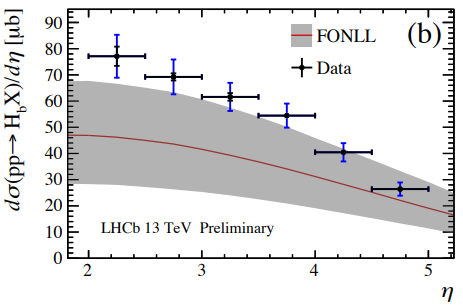
\includegraphics{plots/bbar_forward.png}
  \caption{branching ration of $b$ and $\bar{b}$ production in forward direction. Shown is the data versus fixed-order plus next-to-leading logs(FONLL)\cite{forward}\cite{fonll}.}
  \label{fig:bbforward}
\end{figure}

In this section, a general overview about the requirements for the SciFi Tracker as well as the layout will be discribed based on the presentation in the \textit{technical design report}\cite{scifiInfo} of the upgrade.

The upstream and downstream trackers provide a good precision estimate of the momentum of charged particles so that mass resolution of decayed particles can be precisely measured.
% this is a sentence i used from the TDR!
For particle identification the reconstructed trajectories of charged particles are used as input for the RICH detectors.
The limiting factor for the momentum resolution is multiple scattering for tracks with a momentum lower than $\num{80}\frac{\text{GeV}}{\text{c}}$. For tracks with a higher momentum the detector resolution is the limiting factor.

% why is the scifi there
The SciFi Tracker replaced the inner Tracker (IT) and the outer Tracker (OT)
and is located in the same place as the downstream trackers that were previously installed.

% data and facts
The instantaneous luminosity after the upgrade is expected to be $\SIrange{1}{2e33}{\per\centi\metre\squared\per\second}$ with a bunch spacing of $\SI{25}{\nano\second}$.
The average number of proton-proton interactions per bunch crossing will be between
$\nu = 3.8$ and $\nu = 7.6$.

% layout
\subsection{Layout of the SciFi Tracker}

\begin{figure}
  \centering
  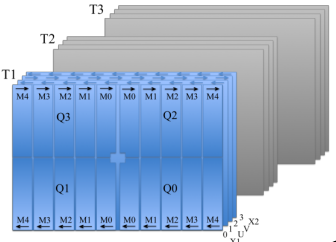
\includegraphics{plots/SciFi_Tracker.png}
  \caption{frontal view of the SciFi geometry and readout order\cite{scifiupdate20210311}.}
  \label{fig:scifi}
\end{figure}

The SciFi Tracker consists of three stations T1, T2 and T3 each having four layers ($X1, U, V, X2$). The orientation of these planes with respect to the vertical axis are ($\SI{0}{\degree}, \SI{+5}{\degree}, \SI{-5}{\degree}, \SI{0}{\degree}$).
Since the beampipe is not exactly parallel to the ground the vertical axis is
defined as vertical on the z-axis of the beampipe.
The tilted layers are called stereo layers and serve the purpose of 3D hit localization.
The layers are $\SI{20}{\milli\metre}$ apart from each other in $z$-direction within each station.
Each layer has four quarters with each quarter having five\footnote{six for the last (T-)station.} modules. Each module is constructed from four fibre mats.
A frontal view of the SciFi Tracker is displayed in figure\ref{fig:scifi}.
The global coordinate system used is of right-handed nature with positive $z$ pointing away from the interaction point following the beam direction as seen in figure \ref{fig:LHCb}. positive $y$ points upwards, towards the surface and positive $x$ and negative $x$ are named as A-Side and C-Side respectivly\cite{scifiInfo}.
For readout purposes the top and bottom half of each element have inverted x- and y-axis as seen in figure \ref{fig:scifi}.

To ensure an optimal alignment, a well known geometry is key. Therefore, the
fibres must be aligned within $\SIrange{50}{100}{\micro\metre}$ in $x$-direction and must not be more than $\SI{300}{\micro\metre}$ bent in $z$-direction.
% here a picture of the scifi

\subsection{Scintillating Fibres}
The scintillating fibre material is a polymer with an organic fluorescent dye
added to the polystyrene structure to enhance the yield during the scintillation process.
In order to produce and register a photon signal, the ionization energy is deposited
in the fibre core firstly. The amount of energy need for the polymer to reach an
excited state is just a few electronvolts. The added dye has the particular structure
to match the excitation energy. The dye generates excited energy states when
particles hit the fibre and deposit their energy.
The long fibre mats and the refractive index make sure total reflection on the inside
happens which guides the photons to the SiPMs\footnote{Silicon Photomultiplier}.
On the opposite end of the SiPM a full reflective mirror is mounted so the photons travelling to the other end do not get lost but reflected towards the SiPM.

%\section{The LHC data cycle}
%\label{sec:datacycle}

\chapter{The Theory of align*ment}
\label{sec:align*Theory}

short introduction

\section{Track reconstruction}
\label{sec:kalman}

In order for LHCb to be used for physics, all of the detector hit information has to be converted into tracks, which is a challenging task.
The track reconstruction algorithm needs to find the correct hits from each subdetector to build the track. This can be problematic just because of the amount of tracks per events (roughly 100).
It is crucial to find all particle tracks and also their track parameters which come from the track fit.

A good track fit is needed in order to find to best estimates for the track parameters and covariances. The estimates are used in the event reconstruction to find the correct tracks for each particle and the decay products. The info provided is used in the RICH rings, ECAL and HCAL and muon detectors. With these information, particle and track parameters such as the invariant mass can be measured and vertex origins can be found.
There are several track models that can be used. In general, a track is build from numerous segments which are either straight or curved because of an active magnetic field. Depending on the environment of the track either model is good.
The track segments are called track states and are defined by a position in $x$ and $y$ at a given distance $z$ where the hit was located, then a tanget direction $t_{x,y}$ at the hit position and a momentum parameter acquired from the track curve inside the magnetic field\cite{VanTilburg}.

In order to correctly reconstruct the track is is important to know where the hit is localized and for the upcoming hits, where to particle track came from. From the momentum measurement of the track curvature caused by the magnetic field, the parameter $q/p$ is also added.

\begin{align*}
  \vec{r} = \left(\begin{array}{c} x \\ y \\ t_x \\ t_y \\ \frac{q}{p}\end{array}\right) &\,\, t_x = \frac{\partial x}{\partial z} & t_y = \frac{\partial y}{\partial z}
\end{align*}

The uncertainty of the five-component state vector is a $5\times5$ covariance matrix $C$.
A track state can be anywhere on the trajectory but is easier to choose it at real detection points. Combining the track state with a real measurement point is called \textit{node}.
The propagation from node $k_{-1}$ to node $k$ is described by a propagation function

\begin{equation*}
  \vec{r}_k = f_k(\vec{r}_{k_{-1}}) + \vec{w}_k\,.
\end{equation*}

This means node $k$ is acquired by propagating node $k-1$ through the propagation function $f_k$ and shifting it by the \textit{process noise} $\vec{w}_k$.
% Process noise can be caused by any scattering phenomenon that may have happened.
LHCb uses process noise to model the scattering.
Depending on the type of propagation, linear or curved, a different propagation function is used.
for a linear extrapolation, $f_k$ results in
\begin{equation*}
  f_k \left(\vec{r}_{k-1}\right) = F_k \vec{r}_{k-1}
\end{equation*}
with the transport matrix $F_k$
\begin{gather*}
  F_K = \begin{pmatrix}
    1 & 0 & \Delta z & 0 & 0 \\
    0 & 1 & 0 & \Delta z & 0 \\
    0 & 0 & 1 & 0 & 0 \\
    0 & 0 & 0 & 1 & 0 \\
    0 & 0 & 0 & 0 & 1 \\
  \end{pmatrix}
\end{gather*}
and $\Delta z$ being the difference in z between the nodes
\begin{equation*}
  \Delta z = z_k - z_{k-1}
\end{equation*}


Trajectory information for each node is provided by the real measurement where the relation between measurement $m_k$ and track state at a given node $k$ is defined as

\begin{equation*}
  m_k = h_k(\vec{r}_k) + \epsilon_k
\end{equation*}

with the projection function $h_k$ and \textit{measurement noise} $\epsilon_k$.
So if the detector only measures the $y$ coordinate of state, the projection function
will be
\begin{equation*}
  h_k(\vec{r}_k) = H_k \vec{r}_k
\end{equation*}
with
\begin{gather*}
  H_k = \begin{pmatrix}
    0 & 1 & 0 & 0 & 0 \\
  \end{pmatrix}
\end{gather*}\,.

When measuring more parameters the measurement matrix $H_k$ and projection matrix have dimension $n\times5$ with $n$ being the numbers of parameters measured.

With this track model, $\epsilon_k$ and $w_k$ are random and unknown and have an expectation value of zero.
% They are defined as $W_k \equiv cov(w_k)$ and $V_k \equiv cov(\epsilon_k)$.

% now kalman filter formalism
\section{The Kalman filter method \cite{VanTilburg}}
In general a track is an ensemble of measurements and track states and the Kalman filter method is used to fit tracks.
The idea of the Kalman filter is, to have a starting node and add measurements one by one. In between the addition of measurements, the local track state is updated with the new information.
The Kalman filter method is a $\chi^2$ minimising problem for the measurement of the track. Because of the iterative nature of the method, it is fast und also used in other fields than physics, for example GPS and meteorology.
The three steps of the Kalman filter will be briefly outlined and later discribed in further detail.


The first step is the $\symbf{Prediction}$: The next track state of the trajectory is predicted based on the track state at the previous node.
The second step is the $\symbf{Filter}$ procedure: By using filter equation*s, the prediction is updated with measurement information in this node. The prediction and filter are repeated for each measurement. With more measurements added, the estimate for the best trajectory is the track state after each filter step.
The final step is called $\symbf{Smoother}$: When the trajectory is complete, smoother equation*s are applied from the last node to the previous node. Therefore the information from all measurements is used in both forward- and backpropagation which results in a more
defined track.

\subsection{first Step: Prediction}
For a given state vector at node \textit{k-1}, the prediction for the $k^{\text{th}}$ state vector and its covariance matrix results from the propagation relations

\begin{align*}
  \vec{r}_p^{k-1} &= f_p\left( \vec{r}_{k-1} \right) \\
  \text{Cov}_k^{k-1} &= F_k C_{k-1} F_k^T + Q_k
\end{align*}

The superscript of the statevector shows the amount of information used in the estimate.
That means $\vec{r}_k^n$ is the smoothed state vector which used all information,
$\vec{r}_k^k-1$ is the predicted state vector and $\vec{r}_k^k \equiv \vec{r}_k$ is the filtered state.

$Q_k$ is the process noise in matrix form and it is part of the predicted
covariance matrix $C_k^{k-1}$.
Because the first state cannot take measurements from the previous state, an initial prediction is taken from the track finding algorithm instead.
The predicted residual between the measurement, $m_k$ and the state vector results in
\begin{equation*}
  \text{res}_k^{k-1} = m_k - h_k\left( \vec{r}_k^{k-1} \right)
\end{equation*}
and the corresponding covariance matrix is defined as
\begin{equation*}
  \text{Cov}_{\text{res},k}^{k-1} = V_k + H_k C_k^{k-1} H_k^T\,.
\end{equation*}

Here, $V_k$ is the measurement variance. With these metrics the minimal $\chi^2$ for the optimal track states can be calculated via
\begin{equation*}
  \left( \chi^2 \right)_k^{k-1} =
  \text{res}_k^{k-1} \left(\text{Cov}_{\text{res},k}^{k-1}\right)^{-1} \text{res}_k^{k-1}
\end{equation*}

\subsection{second Step: Filter}
During the filter step, the track state is updated with the measurement information.
Iteratively, each measurement is added and the filtered state $\vec{r}_k$ and the corresponding covariance matrix is calculated via
\begin{align*}
  \vec{r}_k &= \vec{r}_k^{k-1} + G_p \text{res}+k^{k-1} \\
  \text{Cov}_k &= \left(\mathbb{1} - G_k H_k\right) \text{Cov}_k^{k-1}\,,
\end{align*}
where $G_k$ is the gain matrix of dimension $5\times1$ and is defined as
\begin{equation*}
  G_k = C_k^{k-1} H_k^T \left( \text{Cov}_{\text{res},k}^{k-1} \right)^{-1}
\end{equation*}

Afterwards the residuals and its covariance matrix are calculated and the filtered total $\chi^2$ is defined as
\begin{equation*}
  \left( \chi^2_{\text{filter}} \right)_k = \text{res}_k \text{Cov}_{\text{res},k}^{-1} \text{res}_k\,.
\end{equation*}

The prediction and filter procedure is continued for all measurements until the track is fully reconstructed.
Because the last node at $k \, = \, n$ has the most information in it, a backward update is performed to infuse the previous nodes with the same information as in last node.
This is called \textit{smoother}-step.

\subsection{third Step: Smoother}
The smoother function returns the best possible estimate for track states at
the previous nodes. The method used is called \textit{Rauch-Tung-Striebel}-smoother\cite{RTS}.
The idea is to use backward information and construct a smoothed state vector and covariance matrix
\begin{align*}
  \tilde{r}_k^n &= \vec{r}_k + S_k \left( \vec{r}_{k+1}^n - \vec{r}_{k+1}^k \right) \\
  \tilde{C}_k^n &= C_k
\end{align*}
and the Smoother-matrix $S_k$ of dimension $5\times5$
\begin{equation*}
  S_k = C_k F_{k+1}^T \left( C_{k+1}^p \right)^{-1}\,.
\end{equation*}

In order to calculate the smoothed $\chi^2$ the residual and correspending covariance matrix are
\begin{align*}
  \text{res}_k &= m_k - h_k \vec{h}_k^n \\
  \text{Cov}_{\text{res},k}^n &= V_k - H_k C_k^n H_k^T
\end{align*}

The $\chi^2$ is calculated analogously to the one during the filter step with the difference being the new residuals and covariances.

\section{alignment using derivatives}
\label{sec:derivatives}
% wouter

this will come later. time ran out last week so this will be done later.

%%%%%%% notes %%%%%%%
%wouter pdf. quelle herausfinden!

%martinelli pdf! use some of that information
% -> align*ment is a minimizing problem (chi2) thats why i looked at chi2 plots
%
% -> global translation and sheering motion don't change chi2 values because residuals are unchanged.
%
% -> weak modes: presence of weak modes affect the convergence (poor, takes many iterations), bias in track parameters.
%
% -> most visible weak modes is the "curvature bias" (sophie has mentioned it sometime. must be on one of my sheets)
% also look at twiki!
%
% goals:
% source for now: DPG2021 pdf exact source will be included!

% \begin{enumerate}
%   \item find the best possible configuration of align*ables, degrees of freedom, constraints
%   \item check for weak modes (how? chi2, small eigenvalues)
%   \item null tests as good as possible
%   \item misalign*ment tests to check align*ment
% \end{enumerate}

% main part
\chapter{Alignment of the SciFi}
\label{sec:story}

For the upgrade the LHCb detector was completely rebuilt. In place of the previous IT and OT a new tracking detector was built which utilizes scintillating fibre called SciFi Tracker. The front-end electronics were also upgraded to handle the increasing data rate. For the new SciFi Tracker a new software is used.

Because of the introduction of the new software, the alignment configuration needs to be determined from the beginning. The goal is to find a configuration that can accurately reproduce the position of the real detector and can correct for ``weak modes''.
With some alignment parameters being highly correlated, detector components may move in the same direction or by the same amount. This is called a ``weak mode''. The movements do not affect the alignment $\chi^2$ since the residuals have not changed. Results of weak modes are biases in track parameters and poor alignment convergence.
One of the most visible weak modes is the curvature bias. There a different ways to reduce the effect of weak modes for example using an overlapping detector design or using different data sets to gather more information.

\section{Alignment Configuration}

An alignment configuration is a specific selection of detector elements, alignment parameters, constraints and track- and vertex-selections used for the alignment.
Alignment parameters are the specific degrees of freedom used for the alignment and for each detector element. The Alignment parameters can be any combination of translations and rotations around the $x$, $y$ and $z$ axis($Tx$, $Ty$, $Tz$, $Rx$, $Ry$, $Rz$).
The configuration that produces the best estimate for the detector position is the best candidate and will be used for the Run 3 data taking.
A track and vertex reconstruction is performed before the alignment is evaluated. Depending on the tracks used the output can be different. Mainly two different track selections will be used throughout the thesis shown in table \ref{tab:tracks}

\begin{table}[!ht]
    \centering
    \begin{tabular}{c|c}
        \toprule
            Tracks & Selections \\
        \midrule
            GoodLongTracks &  $P_{\text{total, min}} = \SI{5000}{\mega\electronvolt}$ \\
            & $P_{\text{total, max}} = \SI{200000}{\mega\electronvolt}$ \\
            & $p_\text{T, min} = \SI{200}{\mega\electronvolt}$ \\
            & maximum $\chi^2 = 5$ \\
            & "long" track type \\
            \hline
            HighMomentumTTracks & $P_{\text{total, min}} = \SI{50000}{\mega\electronvolt}$ \\
            & maximum $\chi^2 = 5$ \\
            & "TTrack" track type \\
        \bottomrule
    \end{tabular}
    \caption{SciFi track selection.}
    \label{tab:tracks}
\end{table}

The alignment runs were performed with alignment specific packages from Alignment/Escher and Alignment/TAlignment\cite{align}.
During the alignment, Lagrange constraints can be utilized to minimize alignment
parameter $\alpha $ under the condition
\begin{equation}
  f(\alpha) = 0
\end{equation}
and adding the Lagrange parameter $\lambda$ to get
\begin{equation}
  \Delta \chi^2 = \lambda f(\alpha)\,.
\end{equation}
Lagrange constraints are added to fix loosely constrained degrees of freedom and can be used for any linear combination of translations and rotations as shown in table \ref{tab:lagr}

\begin{table}[!ht]
    \centering
    \begin{tabular}{c|c}
        \toprule
            Tx, Ty, Tz & translation in x, y, z \\
            Rx, Ry, Rz & rotation around x, y, z \\
            Szx, Szy & shearing of x and y along z \\
            Szz, Sxx & scaling in x and z \\
        \bottomrule
    \end{tabular}
    \caption{Lagrange constraints that can be used as alignment parameters.}
    \label{tab:lagr}
\end{table}

An illustration of shearing is shown in figure \ref{fig:shear}.

\begin{figure}
    \centering
    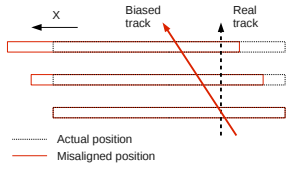
\includegraphics[width=0.6\textwidth]{plots/shearing.png}
    \caption{An illustration of shearing.}
    \label{fig:shear}
\end{figure}

In the software, a Langrange constraint is defined by three elements. A name which can be chosen by the user, the detector element and the alignment parameters, seperated by a colon.

The starting constraints are defined as the following table \ref{tab:cond}, which are based on the alignment conditions from the OT and knowledge from experts.
\begin{table}[!ht]
    \centering
    \begin{tabular}{c | c | c}
        \toprule
            element & positions & uncertainties \\
        \midrule
            $\text{FT}$ & 0 0 0 0 0 0 & 1 1 1 0.0003 0.0003 0.0003 \\
            $\text{FT/T.}$ & 0 0 0 0 0 0 & 1 1 1 0.0003 0.0003 0.0003 \\
            $\text{FT/T./Layer(X1|U|V|X2)}$ & 0 0 0 0 0 0 & 0.2 0.2 0.2 0.0001 0.0001 0.0001 \\
            $\text{FT/.*Module.}$ & 0 0 0 0 0 0 & 0.1 0.1 0.1 0.001 0.001 0.001 \\
            $\text{FT/.*Mat.}$ & 0 0 0 0 0 0 & 0.05 0.05 0.05 0.1 0.1 0.1 \\
        \bottomrule
    \end{tabular}
    \caption{starting condition of the SciFi Tracker.}
    \label{tab:cond}
\end{table}

The SciFi Tracker is referred to as Forward Tracker (FT) in the software.
The first element in each row of the starting conditions is the detector element.
The first set of six numbers are hardcoded parameters for each of the three translation degrees of freedom and three rotational degrees of freedom (Tx, Ty, Tz, Rx, Ry, Rz). They are set to be zero to match the known position of the detector in the Monte Carlo Simulation (MC).
and the second set of six parameters are the corresponding uncertainties.
The scale for the translations are $\si{\milli\metre}$ and the scale for the rotations being $\si{\radian}$. A survey uncertainty of $\num{0.0001}$ stands for $\SI{0.1}{\milli\radian}$.
During this thesis, the LHC beam was off and the SciFi detector was still being constructed. The alignment tests in this thesis use Monte Carlo simulated data to test the alignment software for the SciFi.

\section{Null tests and software tests}
\subsection{Software configurations and samples}
\begin{figure}
  \centering
  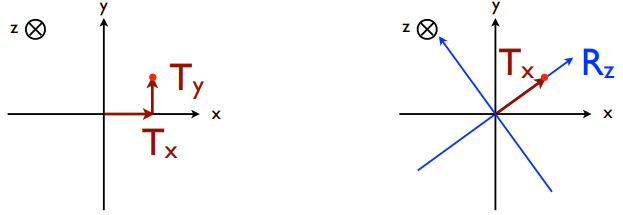
\includegraphics[width=0.75\textwidth]{plots/point_dofs.png}
  \caption{Different ways of describing a measurement point inside the detector(draw this again).}
  \label{fig:dofs}
\end{figure}

At first, a series of tests regarding different degrees of freedom and Lagrange constraints is performed to find the optimal solution for the SciFi Tracker.

The detector layers in the MC are all centered around the beam pipe with no shifting in any direction and the goal is to align the real detector layers to mirror the layers in the software and reduce the shifting as close to zero as possible.

Figure \ref{fig:dofs} is used to demonstrate which degrees of freedom can be used
to describe a point in the detector or a shift in coordinates.
On the left-hand side the measurement point is described through cartesian coordinates and on the right-hand side it is described via polar coordinates.

Problems with the shearing constraints were seen in the VELO alignment, so that a similar analysis for the SciFi was considered.
The parameters used for the VELO were changed to fit the SciFi Tracker and resulted in the following configuration:

\begin{lstlisting}[language=Python]
    dofs = "TxTzRxRz"
    elements.FTStations(dofs)
    elements.FTFrameLayers(dofs)
    TrackSelections = GoodLongTracks()
\end{lstlisting}

The dataset\footnote{upgrade\_DC19\_01\_MinBiasMU} used taken from the TestFileDB\cite{testDB} and will be used for the upcoming tests until a different set is mentioned.
As the DoFs, x- and z-translation as well as rotations around the x- and z-axis are used and are the only relevant DoFs for the alignment since y-translation and rotations around the y-axis can be constructed from the other degrees of freedom.
For the alignment runs, ten iterations were used and is not using input misalignment, so a perfectly aligned detector is expected from the MC.
The alignment constants after each iteration are passed on to the next iteration.
Convergence of the alignment is defined by the difference between the variation of the alignment parameters of the current iteration to the last iteration. If the variation is sufficiently small, the alignment is converged.
The alignable objects are the (T-)stations and the frame layers within a station and the track selection is chosen to be \textit{GoodLongTracks} as a starting point. This will be called \textit{baseline} or \textit{baseline configuration}.
The baseline is unconstrained in order to check the accuracy of the alignment software without constraints and look for weak modes.
The baseline is completely unconstrained.
The frame layers, also called half layers, are divided into two quarters which are the top half and bottom half of the frame layer.

\subsection{Aligning with translations and constraints}
The first configuration tested against the baseline is called “noRotation”. Comparisons of this configuration with the baseline are shown in figure \ref{fig:june_2} and figure \ref{fig:june_2_1}, for 1000 and 7000 simulated events respectively.

In these plots, the measurement points are the mean position of each layer, and the errorbars are root-mean-square errors (RMS) and come from the difference between the C-side and the A-side of the detector layer and is not the measurement uncertainty.
The group position is the global position of the stations and layers inside the LHCb experiment, where $z = 0$ is the far left side of the experiment where the VELO begins.

The "noRotation" configuration is defined as:

\begin{lstlisting}[language=Python]
    dofs = "TxTz"
    elements.FTStations(dofs)
    elements.FTFramelayers(dofs)
    TrackSelections = GoodLongTracks()
    constraints = [
        "station1 : FT/T1 : Tx Tz",
        "station2 : FT/T2 : Tx Tz",
        "station3 : FT/T3 : Tx Tz",
        "frontCSide : FT/T3/Layer(X1|U)/Quarter(0|2) : Tx Tz",
        "backCSide  : FT/T3/Layer(V|X2)/Quarter(0|2) : Tx Tz",
        "frontASide : FT/T3/Layer(X1|U)/Quarter(1|3) : Tx Tz",
        "backASide  : FT/T3/Layer(V|X2)/Quarter(1|3) : Tx Tz"
    ]
\end{lstlisting}

The first three constraints on all stations regarding translations brings the movement of the frame layers within a station to around zero which can be seen clearly in figure\ref{fig:june_2}. The last four constraints restrict the sum of the movement of the half-layers inside each C-frame to be zero, which brings the x translation of the half-layers in station three even closer to zero.
Even though the alignment improved the amount of constraints cannot recover from potential misalignments because the constraints hinder the stations from moving.

In an ideal alignment we want as few constraints as possible so that the alignable objects can be aligned and converge towards the optimal position based on the track reconstruction.
This measurement only used 1000 events and is only used as a guideline to what the trend of the distribution looks like. The associated graphs for $Tx$ plotted against the group position in $z$ are shown in figure \ref{fig:june_2}.

A prominent problem visible is the layer separation between the X-layers and the stereo layers as well as a separation between the C-frames inside each station.

\begin{figure}
  \centering
  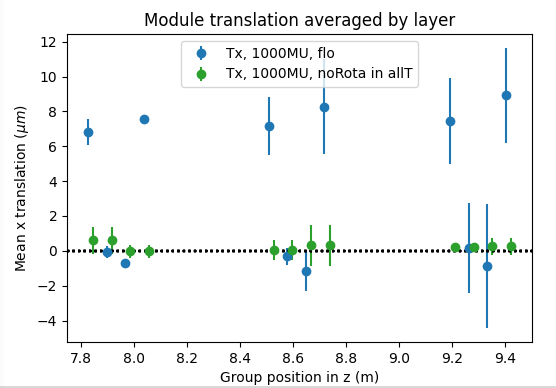
\includegraphics[width=0.8\textwidth]{plots/june_21/Tx_noRota_allT_1000MU.png}
  \caption{comparison of different configurations without rotational constraints in every station, magnet up and 1000 events. plotted is translation in x versus global z.}
  \label{fig:june_2}
\end{figure}

\begin{figure}
  \centering
  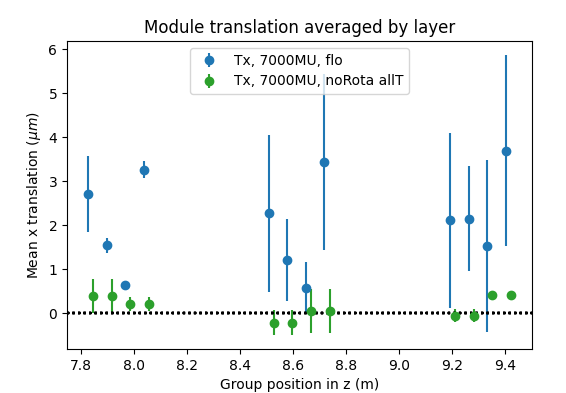
\includegraphics[width=0.8\textwidth]{plots/june_21/Tx_noRota_allT_7000MU.png}
  \caption{comparison of different configurations without rotational constraints in all stations, magnet up and 7000 events. plotted is x translation versus global z.}
  \label{fig:june_2_1}
\end{figure}

In figure \ref{fig:june_2_1} the same measurement was performed for 7000 events to get a better picture. In comparison to \ref{fig:june_2} an overall improvement of the baseline is visible and the layer-splitting is reduced but still prominent. The green measurement shows no direct improvement since the layers are already pretty close to zero in x-direction.
Using 7000 events instead of 1000 events showed a more realistic picture but
took more time to compute especially for 10 alignment iterations.
For the following configuration, 3000 simulated events were used to shorten the computing time while still yielding an accurate representation of the situation.

% for comparisons include the 3000MU plot from renewed_plots
\subsection{Aligning with translations, rotations, and constraints}
The next configuration tested will be called "half C-frame". This configuration is defined as

\begin{lstlisting}[language=Python]
    dofs = "TxTzRxRz"
    elements.FTStations(dofs)
    elements.FTFramelayers(dofs)
    TrackSelections = GoodLongTracks()
    constraints = [
        "station1 : FT/T1 : Tx Tz",
        "station2 : FT/T2 : Tx Tz",
        "station3 : FT/T3 : Tx Tz",
        "frontCSide : FT/T3/Layer(X1|U)/Quarter(0|2) : Tx Tz : total",
        "backCSide  : FT/T3/Layer(V|X2)/Quarter(0|2) : Tx Tz : total"
]
\end{lstlisting}

The degrees of freedom used for this configuration are the same as in the baseline configuration for the same reason.
We chose to align the stations in the given DoFs to fix their overall position in the SciFi and also align the half-layers since we see a separation between the layers which we want to correct with the following constraints.
The stations are constrained in $Tx$ and $Tz$ to fix the overall movement inside the SciFi. The second to last constraint (``frontCSide´´) is constraining the first to half-layers in station three in their total movement along the x- and z-axis.
The last constraint works the same but for the back two half-layers of station three.

and the comparison to the baseline is shown in figure \ref{fig:june_3}.
Here the stations and layers are aligned in $Tx$, $Tz$, $Rx$ and $Rz$ but the stations are still only constrained in their translations. Also, the last station only has one side of each C-frame constrained. The additional keyword \textbf{total} constraints
the difference of the quarters to zero with respect to the nominal position. As seen in figure \ref{fig:june_3} the first two layers have an average position of zero but the individual position is not. The same is seen in the last two layers of each station.

This new configuration in orange converged after 12 iterations as seen in figure \ref{fig:conv}.
This figure shows the mean of the modules in each station per iteration. The modules of station one are the (colour1) dots, the modules for station two are coloured (colour2) and for station three is coloured (colour3).
The horizontal red line is the nominal position of the SciFi in MC, where the aligned detector should be.
The blue, dotted, vertical line marks the point of convergence for the alignment run.
Normally, an alignment job should converge after three to five iterations. If the convergence happens later there could be a problem with the constraints which prevent the alignment from converging because they are implemented wrongly, are redundant or weak modes hinder the convergence.

\begin{figure}
  \centering
  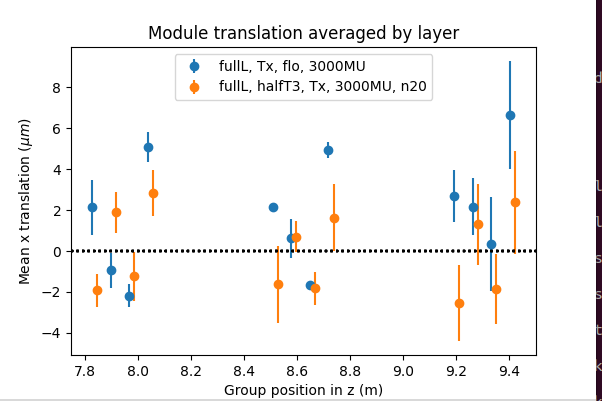
\includegraphics[width=0.8\textwidth]{plots/june_21/allT_halfT3_n20_Tx.png}
  \caption{analysed 20 iterations for x translation behavior for configuration "half C-frame".}
  \label{fig:june_3}
\end{figure}

\begin{figure}
  \centering
  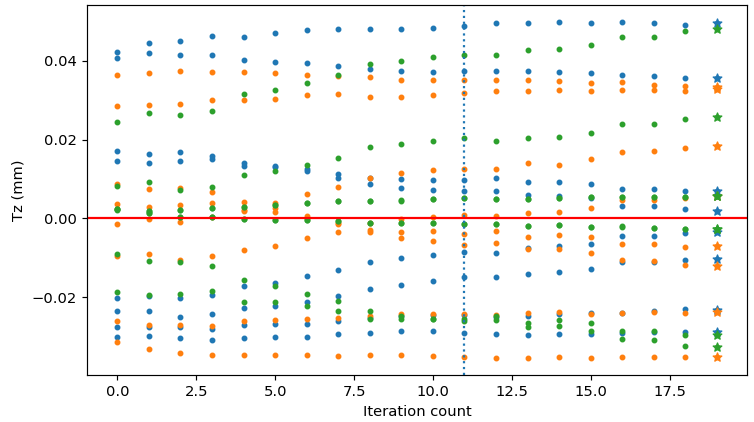
\includegraphics[width=0.75\textwidth]{plots/scatter_fig_4_4_convergence.png}
  \caption{convergence of the alignment after 12 iterations from configuration "half C-frame".}
  \label{fig:conv}
\end{figure}

\section{Null tests with rotational constraints}
In the previous section rotations were not used inside the constraints. Now the constraints will include rotational constraints and test the changes.

Similar to the "noRotation" configuration the same constraints were used but for different degrees of freedom. The new configuration is called "Full DoF" which uses every degree of freedom and is defined as:

\begin{lstlisting}[language=Python]
    dofs = "TxTyTzRxRyRz"
    elements.FTStations(dofs)
    elements.FTFramelayers(dofs)
    TrackSelections = GoodLongTracks()
    constraints = [
        "station1 : FT/T1 : Tx Ty Tz Rx Ry Rz",
        "station2 : FT/T2 : Tx Ty Tz Rx Ry Rz",
        "station3 : FT/T3 : Tx Ty Tz Rx Ry Rz",
        "frontCSide : FT/T3/Layer(X1|U)/Quarter(0|2) : Tx Ty Tz Rx Ry Rz",
        "backCSide  : FT/T3/Layer(V|X2)/Quarter(0|2) : Tx Ty Tz Rx Ry Rz",
        "frontASide : FT/T3/Layer(X1|U)/Quarter(1|3) : Tx Ty Tz Rx Ry Rz",
        "backASide  : FT/T3/Layer(V|X2)/Quarter(1|3) : Tx Ty Tz Rx Ry Rz"
        ]
\end{lstlisting}

In figure \ref{fig:june_4} x-translation and z-translation with regards to the group position are shown.

\begin{figure}
  \centering
  \begin{subfigure}[b]{0.4\textwidth}
    \centering
    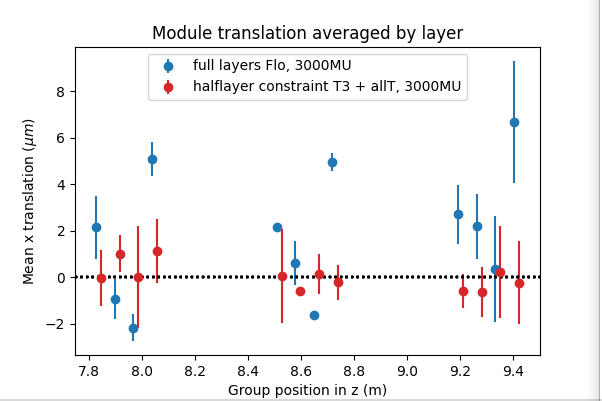
\includegraphics[width=\textwidth]{plots/june_21/allT_halfT3_Tx_vs_Flo.png}
    \caption{x-translation versus group position in z.}
    \label{fig:june_4_1}
  \end{subfigure}
  \hfill
  \begin{subfigure}[b]{0.4\textwidth}
    \centering
    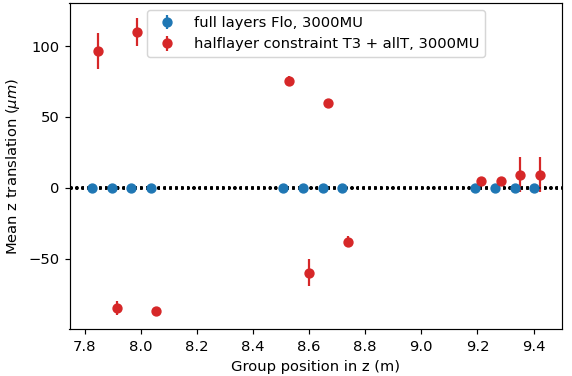
\includegraphics[width=\textwidth]{plots/scatter_fig4_2.png}
    \caption{z-translation versus group position in z.}
    \label{fig:june_4_2}
  \end{subfigure}
  \caption{"Full DoF" configuration (red) plotted versus baseline configuration (blue) for 3000 events.}
  \label{fig:june_4}
\end{figure}

Figure \ref{fig:june_4_1} still shows layer separation in station 1 more similar to figure \ref{fig:june_3} than to figure \ref{fig:june_2_1}.
Since the constraints are the same and the amount of degrees of freedoms increased,
it is visible that using more DoFs makes the alignment worse. Therefore the degrees of freedom must be chosen wisely.

Regarding the z-translation the plot is only shown to demonstrate the large separation of layers. the baseline was not aligned in $Tz$ so there is no comparison.

The RMS uncertainty on the measurements is a result of the separation between A-side and C-side. For configuration "Full DoF", a plot showing the C-side and A-side difference in x-translation is presented in figure \ref{fig:june_5} and for z-translation in figure \ref{fig:june_6}.

A clear layer separation is visible in terms of layer translation along the beam pipe\ref{fig:june_5}.
The first and third layer in each station move away from the IP and the second and
fourth layer move towards the IP.
Because of the many constraints that are applied to T3, the RMS uncertainty in the other stations get worse. Because the last station is overconstrained the track reconstruction moves the other stations accordingly which results in a larger RMS uncertainty for the half-layers in station 1 and 2.

\begin{figure}
  \centering
  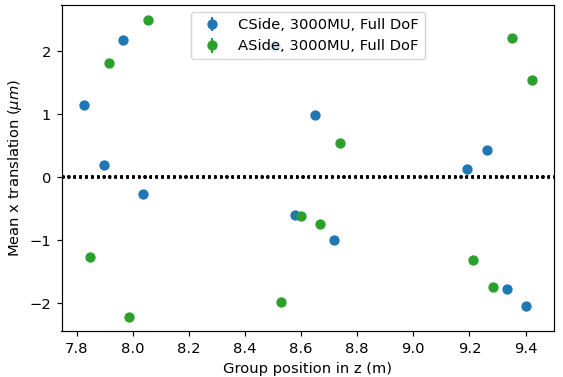
\includegraphics[width=0.8\textwidth]{plots/renewed_plots/CA_allT_halfT3_Tx.png}
  \caption{compare C-Side to A-Side for translation in x direction.}
  \label{fig:june_5}
\end{figure}

\begin{figure}
  \centering
  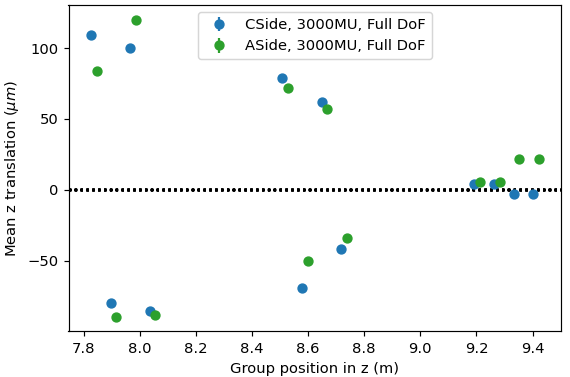
\includegraphics[width=0.8\textwidth]{plots/renewed_plots/CA_allT_halfT3_Tz.png}
  \caption{compare C-Side to A-Side for translation in z direction.}
  \label{fig:june_6}
\end{figure}

The x-translation in Figure \ref{fig:june_5} also shows some separation, the last two layers in station 3 are separated from the first two regarding z-translation. Especially the half-layers in the last station should be fixed around zero with the constraints added. The sum of all translations should be zero with each individual layer movement being small.

This result is unexpected with the constraints added. In the next sections, more tests are described, while the underlying cause of these unexpected results is described in Section \ref{sec:clusterbias}.

\subsection{Checking rotational degrees of freedom}
\label{sec:test_and_c5}
The Next configuration tested is the result of a series of tests with various constraints, DoFs and alignable objects. In figure \ref{fig:TxZ} a new configuration called "Test3" is introduced and it is defined as

\begin{lstlisting}[language=Python]
dofs = "TxTzRxRz"
elements.FTStations(dofs)
elements.FTFramelayers(dofs)
TrackSelections = GoodLongTracks()
constraints = [
    "station3 : FT/T3 : Tx Tz Rx Rz",
    "frontCSide : FT/T3/Layer(X1|U)/Quarter(0|2) : Tx Tz Rx Rz",
    "backCSide  : FT/T3/Layer(V|X2)/Quarter(0|2) : Tx Tz Rx Rz",
    "frontASide : FT/T3/Layer(X1|U)/Quarter(1|3) : Tx Tz Rx Rz",
    "backASide  : FT/T3/Layer(V|X2)/Quarter(1|3) : Tx Tz Rx Rz"
    ]
\end{lstlisting}

\begin{figure}
  \centering
  \begin{subfigure}[b]{0.4\textwidth}
    \centering
    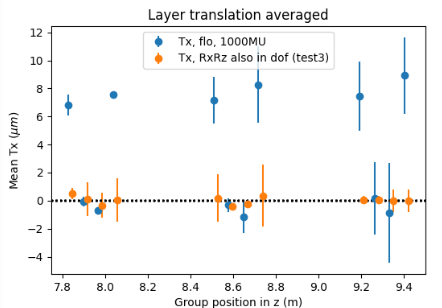
\includegraphics[width=\textwidth]{plots/july_28/Tx.png}
    \caption{x-translation versus group position in z.}
    \label{fig:TxZ_1}
  \end{subfigure}
  \hfill
  \begin{subfigure}[b]{0.4\textwidth}
    \centering
    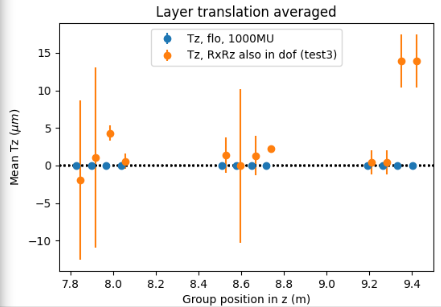
\includegraphics[width=\textwidth]{plots/july_28/Tz.png}
    \caption{z-translation versus group position in z.}
    \label{fig:TxZ_2}
  \end{subfigure}
  \caption{"Test3" configuration (orange) plotted versus baseline configuration (blue) for 1000 events.}
  \label{fig:TxZ}
\end{figure}

Here the last four C-frame constraints have rotational degrees of freedom added.
Looking at \ref{fig:TxZ_1} each station has a quite low movement in x-direction comparing to the previous configurations. In the last station, the first two layers the C-side and A-side are exactly where they should be inside the detector since the RMS is very close to zero. The last two layers only show a small uncertainty. In station
two the X-layers are separating from the stereolayers. The X-layers also have a noticable RMS uncertainty. In this configuration the degrees of freedom are chose in a way for the alignment to either use them as two pairs of cartesian coordinates (Tx Tz, and Rx Rz) or interpret them as two pairs of polar coordinates (Tx Rz and Tz Rx).
This and also the reduction in constraints seemed to help the alignment in terms of x-translation, not so much regarding z-translation. Also this plot only shows the alignment for 1000 events and 10 iterations but overall an improvement was achieved
when it comes to constructing a good configuration.

The next configurations are called "config5" (blue) and "config5 Rz" (orange). The plots showing the translations are shown in figure \ref{fig:config5_tra} and the rotations are shown in figure \ref{fig:config5_rot}.
The blue measurement has the same constraints as "Test3" with an added back C-frame constraint:
\begin{lstlisting}[language=Python]
  constraints.append("back_C_frame_T3 : FT/T3/Layer(V|X2) : Tx Tz")
\end{lstlisting}

The orange measurement has a similar constraint added with Rz added to the DoFs inside the constraint:
\begin{lstlisting}[language=Python]
  constraints.append("back_C_frame_T3 : FT/T3/Layer(V|X2) : Tx Tz Rz")
\end{lstlisting}

Comparing just these two configurations, regarding $Tx$ there is not a big difference.
The last station has a little more separation in "config5 Rz", station 2 shows roughly the same performance and station one is also more split, in total approximately
$\SI{0.5}{\micro\metre}$. The overall z-translation regressed by a small amount in every station while the layer spearation in station 3 improved.
It can be seen, that both X-layers in T2 in the x-translation plot have a quite large RMS uncertainty which means the A-side and the C-side in the X-layers are quite far apart but the mean is right around 0. That is expected since the constraint added only brings the mean of the layer to 0. In future analyses new constraints will be added to bring the sides together.
% config 5
\begin{figure}
  \centering
  \begin{subfigure}[b]{0.4\textwidth}
    \centering
    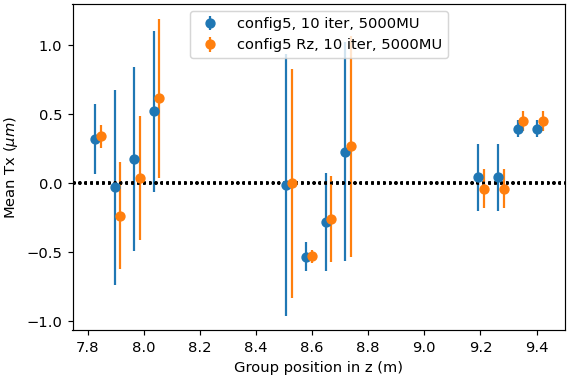
\includegraphics[width=\textwidth]{plots/renewed_plots/Tx_config5.png}
    \caption{x-translation versus group position in z.}
    \label{fig:config5_Tx}
  \end{subfigure}
  \hfill
  \begin{subfigure}[b]{0.4\textwidth}
    \centering
    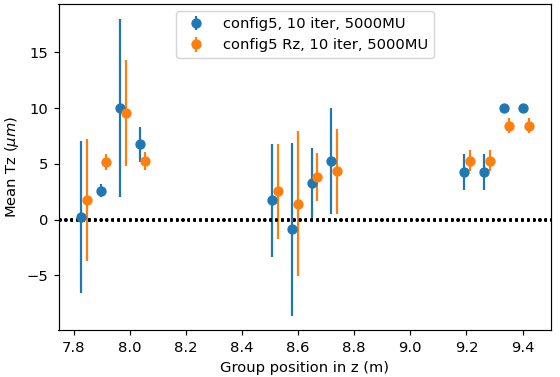
\includegraphics[width=\textwidth]{plots/renewed_plots/Tz_config5.png}
    \caption{z-translation versus group position in z.}
    \label{fig:config5_Tz}
  \end{subfigure}
  \caption{"config5" configurations (blue) plotted versus "config5 Rz" configuration (orange) for 5000 events.}
  \label{fig:config5_tra}
\end{figure}

Rotations around $x$ will not be further analysed because it does not have a huge impact on the alignment quality and is also very well aligned. In $Rz$ a noticable gap
between the two measurements can be seen. This is a result from the added $Rz$ constraint on the last two layers.
The constraints used should result in a rotation smaller than what is seen in figure \ref{fig:config5_Rz}.
A possible cause for that can be a bias inside the SciFi hit clusters and will be discussed later in section \ref{sec:clusterbias}.

\begin{figure}
  \centering
  \begin{subfigure}[b]{0.4\textwidth}
    \centering
    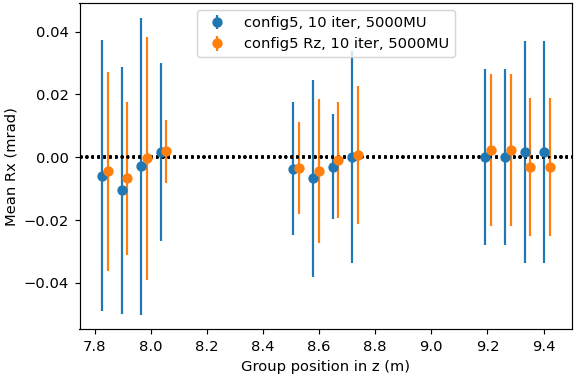
\includegraphics[width=\textwidth]{plots/renewed_plots/Rx_config5.png}
    \caption{x-rotation versus group position in z.}
    \label{fig:config5_Rx}
  \end{subfigure}
  \hfill
  \begin{subfigure}[b]{0.4\textwidth}
    \centering
    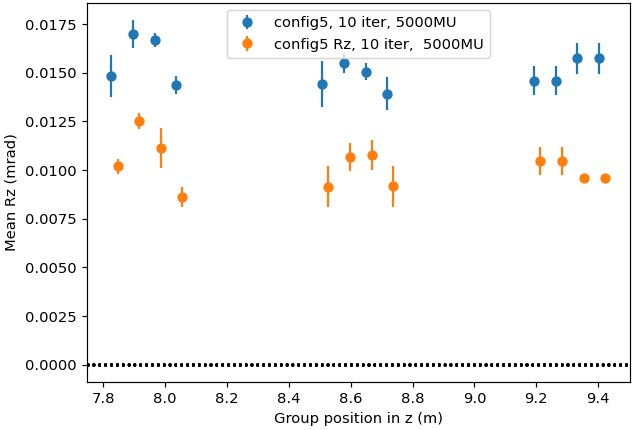
\includegraphics[width=\textwidth]{plots/renewed_plots/Rz_config5.png}
    \caption{z-rotation versus group position in z.}
    \label{fig:config5_Rz}
  \end{subfigure}
  \caption{"config5" configurations (blue) plotted versus "config5 Rz" configuration (orange) for 5000 events.}
  \label{fig:config5_rot}
\end{figure}

Regarding the goal to reduce the amount of rotation and translation in each station,
the result is a small improvement in $Rz$ of around $\SI{0.005}{\milli\radian}$ in every layer. $Rx$ is mostly unchanged as well as $Tx$.

Translation constraints as well as rotation constraints are not the only constraints tested. There are also scaling- and shearing constraints that were tested but seemed to have no major impact.

\section{chi2 tests and weak modes}
In this section, a $\chi^2$ analysis is performed in order to study the ``goodness'' of the alignment and determine the impact of potential weak modes also known as "correlated alignment parameters". There are several weak modes that could occur namely \textit{global translation}, \textit{shearing} and \textit{curvature bias}.
Weak modes are unaffected by the $\chi^2$ since the residuals do not change but they do however show in terms of the eigenvalues of track parameters.
The effect weak modes have on the alignment are biases regarding track parameters and late convergences.
There are different solutions that can be utilized to reduce the effect from weak modes such as
\begin{itemize}
  \item $\textbf{using other data-taking configurations like magnet off or mass plots \\for off-axis events}$
  \item $\textbf{utilizing other survey data sets}$
  \item $\textbf{using kinematic and vertex constraints}$
\end{itemize}\,.

Using magnet-off data can be helpfull as a comparison measurement since it can be utilized to constrain the curvature bias, which will not be element of this thesis but for future analyses.

\begin{figure}
  \centering
  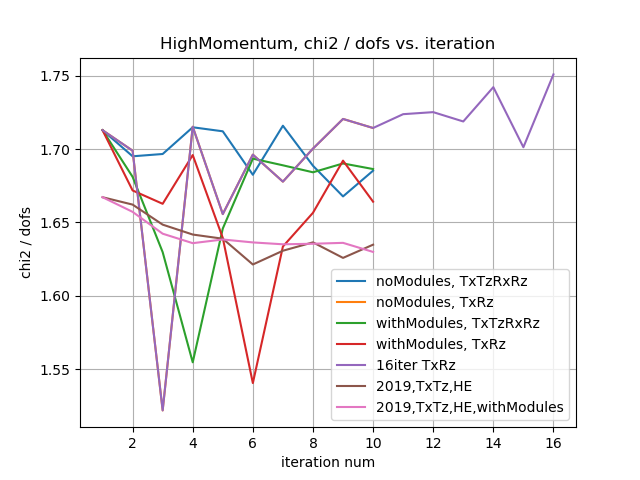
\includegraphics[width=0.8\textwidth]{plots/nov_19/Figure_2.png}
  \caption{$\chi^2 / dofs$ versus iteration number of different degrees of freedom, alignables and data samples.}
  \label{fig:fig2}
\end{figure}

The first test is the $\chi^2$-analysis for \textit{HighMomentumTTracks},
6500 events and 2020 data plotted versus the iteration number during the
alignment in figure \ref{fig:fig2}.
This track selection was chosen because TTracks are mainly produced in secondary interactions and are identified by only having hits inside the T-stations as seen in figure \ref{fig:tracksel}.
\begin{figure}[!ht]
    \centering
    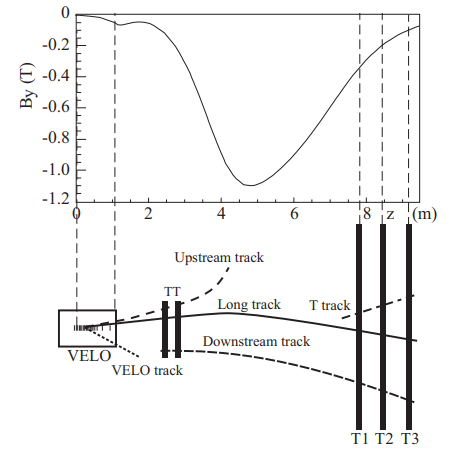
\includegraphics[width=0.8\textwidth]{plots/track_selection.png}
    \caption{An illustration of different track types as well as the main B-field component ($B_y$) as a function of the $z$ coordinate.}
    \label{fig:tracksel}
\end{figure}
Since the main B-field component is quite large inside the T-stations, \textit{HighMomentumTTracks} are especially useful for studies regarding magnet-off data because the difference between magnet-on and magnet-off is large.
These measurements are interesting to compare with studies regarding the curvature bias in future analyses.
In blue, stations and layers were aligned in $Tx$,
$Tz$, $Rx$ and $Rz$ with the constraints being used from "config5" from section \ref{sec:test_and_c5}. The orange
measurement is identical except for the degrees of freedom being only $Tx$ and $Rz$.
In green and red the same measurements as in blue and orange were performed with
the difference that that the modules are aligned as well.
The purple measurement is the only one which covers 16 iterations and is otherwise identical to the orange one. That is also why the orange measurement is not visible since it lies behind the purple one for the first 10 iterations.
the brown and pink measurements are done for simulated data with an older description of the detector geometry from 2019, and are otherwise identical to the orange and red measurement regarding constraints and alignable degrees of freedom.

The spiky behavior in this plot is not what we expected and this might be the result of weak modes since the convergence is quite bad in all of the 2020 data which can be seen by the $\chi^2 / dofs$ not steadily decreasing.
The 2019 measurements were performed as control measurements with and without
module alignment. Here a clear decrease in the $\chi^2 / dofs$ is visible. This
indicates that for the 2020 MC sample additional analysis must be performed to gain further knowledge about the MC data set since it shows some unclear findings.

The idea to test $Tx$, $Tz$, $Rx$ and $Rz$ versus only one translation and one
rotational degree of freedom was to analyse the effect regarding the convergence and the $\chi^2 / dofs$ itself. One could also argue that there was a quick convergence after three iterations when looking at the yellow measurement but something happened afterwards. This will be analysed in a future project.

In figure \ref{fig:chi2iter} a comparison between GoodLongTracks and HighMomentumTTracks for the same measurements was performed to to study the impact of different track selections. This shows, that the alignment quality for both track selections increases with the number of iterations.
The identical $\chi^2$ measurements for the HighMomentumTTracks were plotted against the number of tracks as seen in figure \ref{fig:chi2tracks} as an example.
A clear correlation between the $\chi^2 \ \text{dofs}$ and the number of tracks can be seen.

\begin{figure}
  \centering
  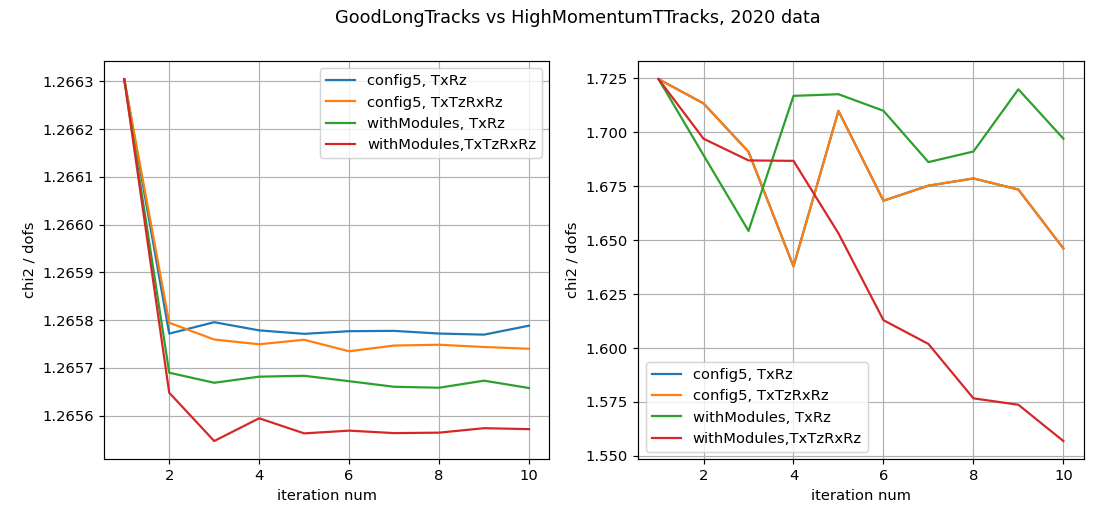
\includegraphics[width=0.8\textwidth]{plots/GL_HM_chi2_2020.png}
  \caption{$\chi^2$-test versus number of tracks of different degrees of freedom, alignables and data samples.}
  \label{fig:chi2iter}
\end{figure}

\begin{figure}
  \centering
  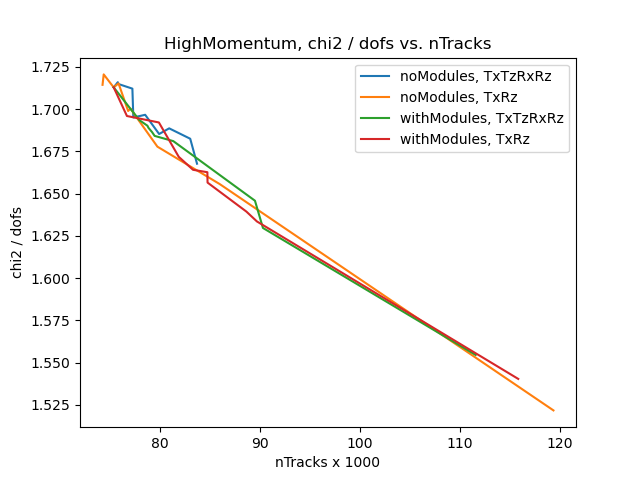
\includegraphics[width=0.8\textwidth]{plots/nov_21/chi2_vs_ntracks_all.png}
  \caption{$\chi^2$-test versus number of tracks of different degrees of freedom, alignables and data samples(redo with grid).}
  \label{fig:chi2tracks}
\end{figure}

\begin{figure}
  \centering
  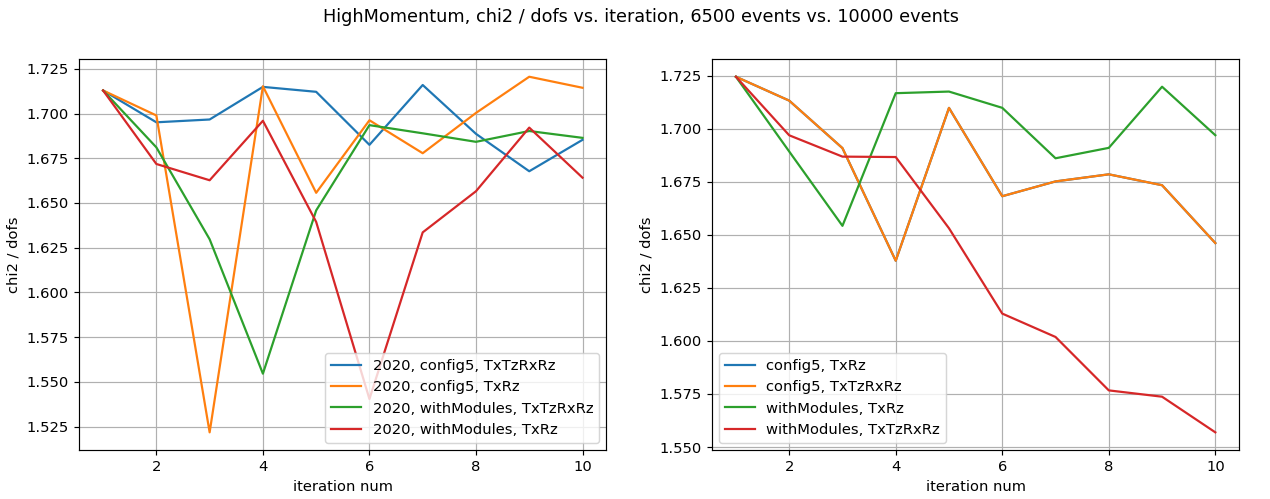
\includegraphics[width=\textwidth]{plots/LHCB_week_dec/chi2_vs_iter_normal.png}
  \caption{$\chi^2 / dofs$ versus iteration number for different number of events.}
  \label{fig:chi2iterdec}
\end{figure}

In figure \ref{fig:chi2iterdec} a side-by-side view of the same $\chi^2$ measurement
is shown but for different number of events. Despite the different labels these are the same measurements, only the colors are switched around for red and green and also yellow and blue as a pair. The thing that strikes the eye is the steadily decrease in $\chi^2 / dofs$ in the red measurement. Unlike our first expectations that $Tx$ and $Rz$ are enough degrees of freedom to describe the system using additional degrees of freedom seemed to help the alignment.
Also, the blue measurement sits behind the orange which might be due to an
programming error.

In figure \ref{fig:chi2tracksdec} a consistency check for figure
\ref{fig:chi2iterdec} was performed. The number of tracks correlate well with
the $\chi^2 / dofs$.
% The blue measurement is missing again which seems to be a programming error.

\begin{figure}
  \centering
  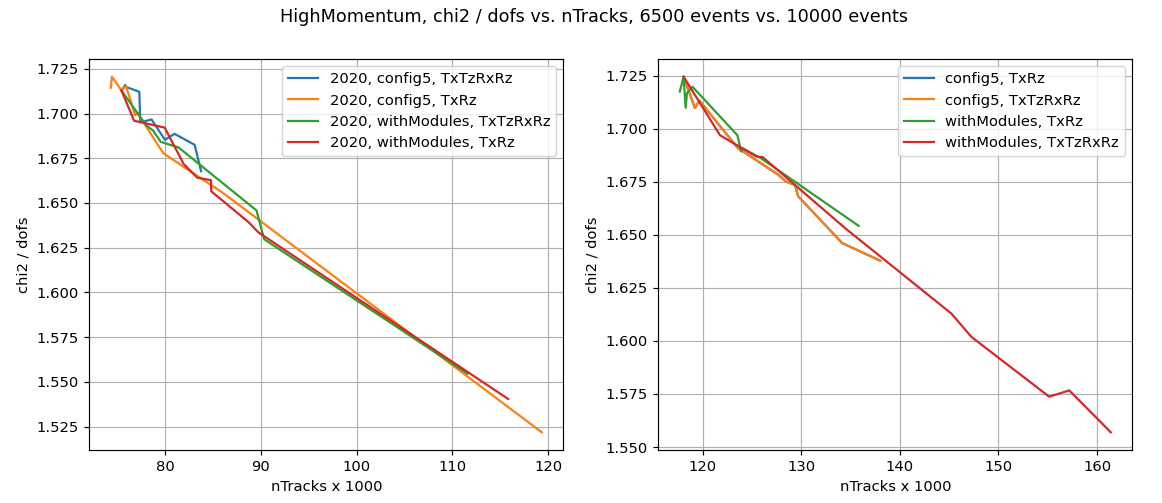
\includegraphics[width=\textwidth]{plots/LHCB_week_dec/chi2_vs_tracks_normal.png}
  \caption{$\chi^2 / dofs$ versus number of Tracks for 6500 events and 10000 events.}
  \label{fig:chi2tracksdec}
\end{figure}

We found out that the MC sample from 2020 using the newer detector geometry contains some aspects that require more tests for example the spikey behavior of the $\chi^2 / \text{dof}$. Figure \ref{fig:chi2iter} shows the same measurements for GoodLongTracks in comparison to HighMomentumTTracks which made it even more clear that the MC sample from 2020 is problematic. The GoodLongTracks shows an early convergence which is good. It also shows that aligning the modules of the SciFi instead of the stations and the half-layers is slightly better for the alignment performance. Hints of potential weak modes could be the problem in the 2020 MC samples shown by the late convergence and the irregular behavior in the $\chi^2$ tests.

\section{luminosity samples and chi2}
In order to get a clearer view of the difference in alignment quality, coming from the difference in luminosity during the ramp-up phase and the data taking phase, samples of different luminosities are looked at.
Comparing two samples, one with a "ramp-up" luminosity with a parameter $\nu = 3.8$ also referred to as "low luminosity" and one for the luminosity used during the data taking
with $\nu = 7.6$, called "normal luminosity".
The $\chi^2 / dofs$ of these samples is plotted versus the iteration number \ref{fig:chi2iter_lumi_normal} and the number of tracks\ref{fig:chi2tracks_lumi_normal}.

in figure \ref{fig:chi2iter_lumi_normal} we see the expected convergence after iteration three and a quite low $\chi^2 / dofs$ of around $\num{1.28595}$ for the normal luminosity sample
and $\num{1.3067}$ for the low luminosity sample.

\begin{figure}
  \centering
  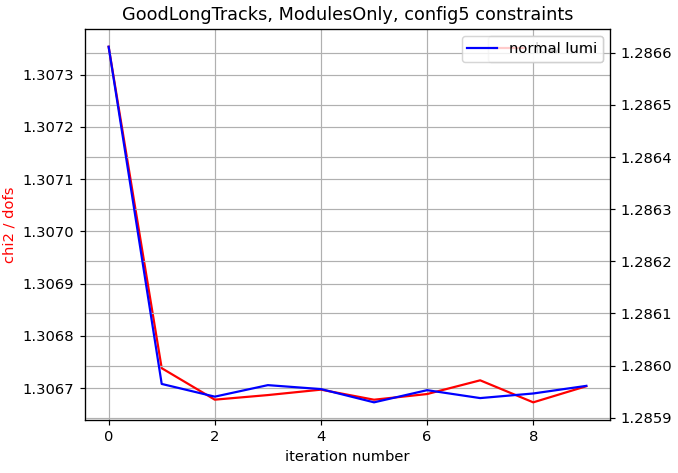
\includegraphics[width=0.8\textwidth]{plots/renewed_plots/modules_chi2_c5.png}
  \caption{compare different luminosities and plot $\chi^2$ versus iteration number.}
  \label{fig:chi2iter_lumi_normal}
\end{figure}

\begin{figure}
  \centering
  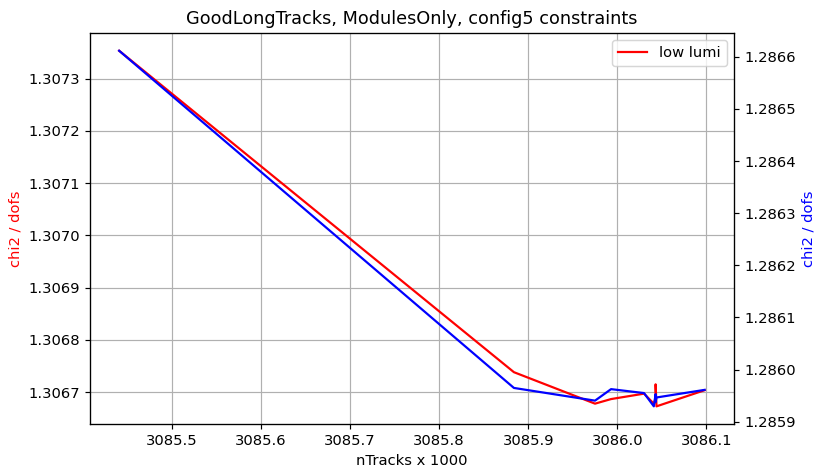
\includegraphics[width=0.8\textwidth]{plots/jan_17_2022/chi2_tracks_modulesOnly.png}
  \caption{compare different luminosities and plot $\chi^2$ versus number of tracks as a measurement for weak modes and alignment.}
  \label{fig:chi2tracks_lumi_normal}
\end{figure}

This short study shows, that the difference in alignment quality coming from different luminosities is small, which can be seen in the difference in $\chi^2 / \text{dofs}$. For both samples the convergence happend early, which is expected.

\section{impact of the cluster bias}
\label{sec:clusterbias}

As mentioned earlier the cluster bias most certainly causes the shift in the rotation around $z$ for each layer so it does not reach 0.
To test that a momentary fix was found and implemented. The workaround was to add a scaling for the \textit{m\_airgap}\cite{gap}.

Figure \ref{fig:cbhack_on_off} shows the impact of the cluster bias fix regarding the rotation around $z$.

\begin{figure}
  \centering
  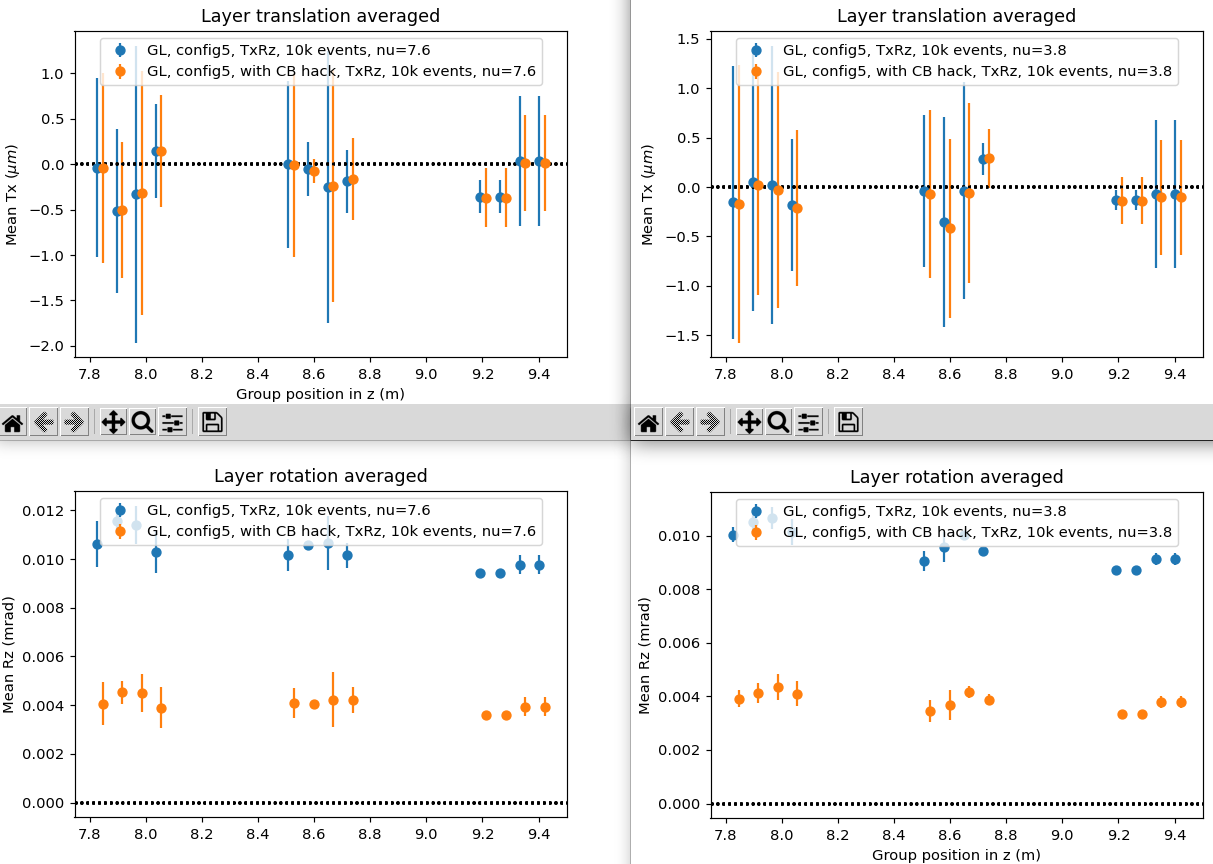
\includegraphics[width=0.8\textwidth]{plots/jan_24_2022/compare_with_without_hack.png}
  \caption{Impact of the clusterbias for high and low luminosity samples.}
  \label{fig:cbhack_on_off}
\end{figure}

As we expected, the amount of rotation was reduced to about
$\SI{0.004}{\milli\radian}$ from the previous $\SI{0.01}{\milli\radian}$ which is more than a factor of 2 improvement. Because the rotation still does not reach zero, we know that this is not a true fix for the cluster bias, and further analysis will be needed to find the true source. That analysis is beyond the scope of this thesis.

Now that we know that the cluster bias can be reduced we take a closer look at samples of different luminosities since the LHC will not be operated at the maximum luminosity from the start, there is also the ramp up phase where the luminosity will be lower.

Since we want to know what the shifts in rotation and translation will look like when the cluster bias is fixed we will keep the fix active for the next studies.
Figure \ref{fig:lumi_low_normal_hack_on} shows the difference between a sample with ramp-up luminosity and a sample with the luminosity during the measurement phase.
We see, that the layer separation is much more prominent in station 1 and 3 for the higher luminosity sample but slightly better behaved in station 2 when looking at x-translation.
Regarding the z-rotation, the lower luminosity sample as slightly lower rotational shifts.
The difference is so minute that it can be safely disregarded. (not sure about that)

\begin{figure}
  \centering
  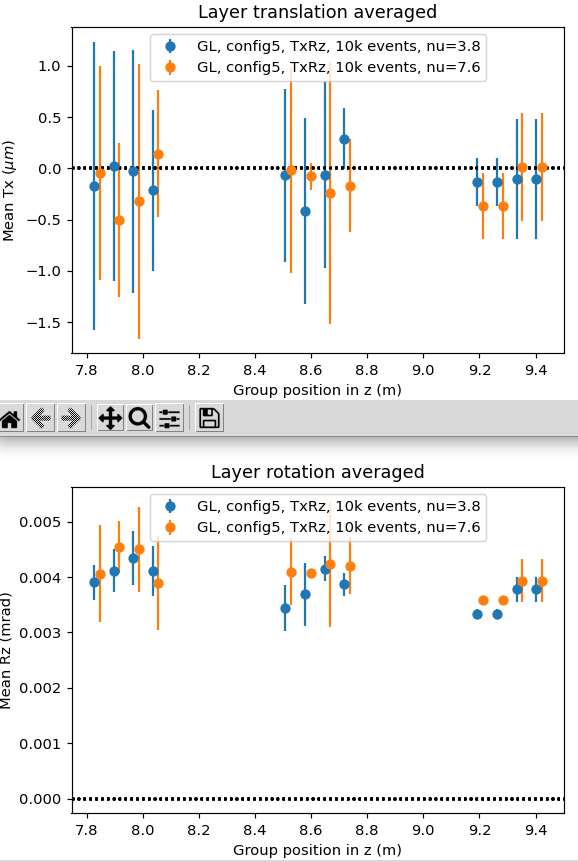
\includegraphics[width=0.8\textwidth]{plots/jan_24_2022/low_normal_with_hack.png}
  \caption{show difference between low and normal luminosity with clusterbias fix active.}
  \label{fig:lumi_low_normal_hack_on}
\end{figure}

With that, we tested if there is a noticable difference in the $\frac{\chi^2}{\text{dof}}$
and the result is shown in figure \ref{fig:GL_lumi_low_normal_hack_on}.

\begin{figure}
  \centering
  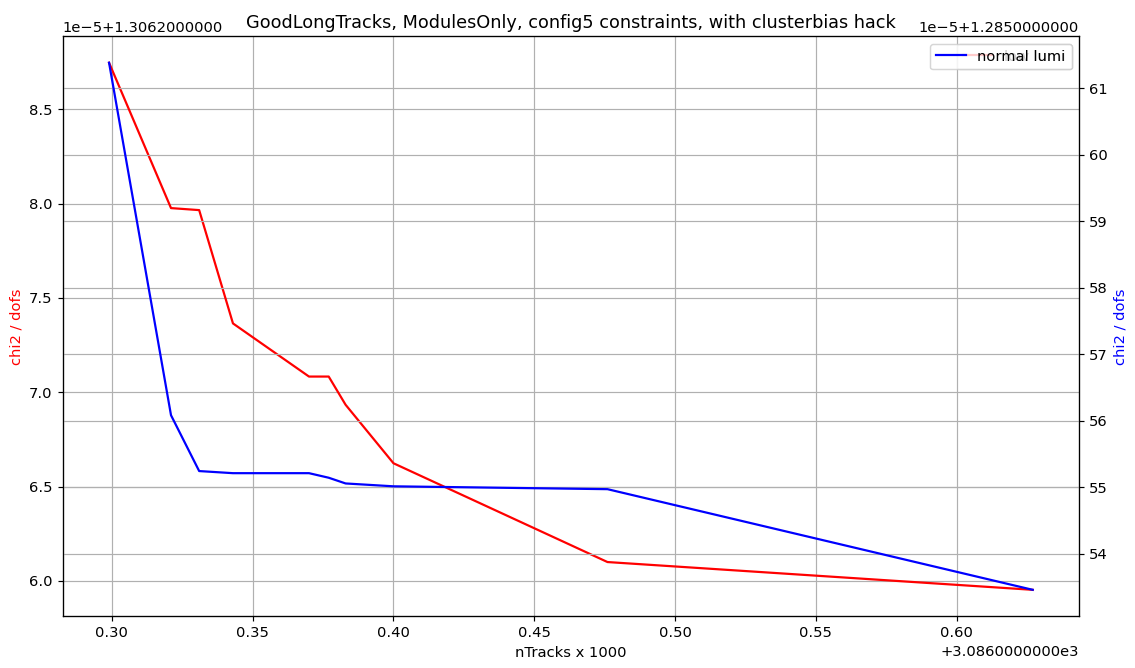
\includegraphics[width=0.8\textwidth]{plots/feb_2_2022/GL_modules_c5_cb_hackactive_low_normal_lumi.png}
  \caption{GoodLong tracks for module alignment and config 5 active. also the clusterbias fix is active comparing low and normal luminosity.}
  \label{fig:GL_lumi_low_normal_hack_on}
\end{figure}

\begin{figure}
  \centering
  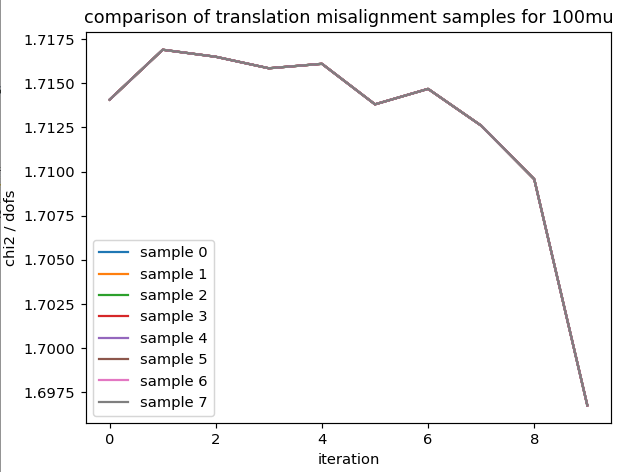
\includegraphics[width=0.8\textwidth]{plots/feb_6_2022/100mu_misalignment_samples_compared.png}
  \caption{100mu translation misalignment comparison for different misalignment samples.}
  \label{fig:100muT}
\end{figure}

Now, since the alignment works quite good with the current configuration we
tested how translation misalignment effects the convergence by looking at the
$\chi^2$, portrayed in figure \ref{fig:100muT}. For this figure, eight different samples of $\SI{100}{\micro\metre}$ module translation misalignment over all translatory
degrees of freedom. The idea behind using different samples is to reduce errors
from biased samples. The plot shows the total $\chi^2$ over degrees of freedom
plotted against the number of iterations. We see no visible difference regarding
the total $\chi^2$ between the samples which is good.
Also, the total $\chi^2$ decreases with an increasing number of iterations
during the alignment.

\begin{figure}
  \centering
  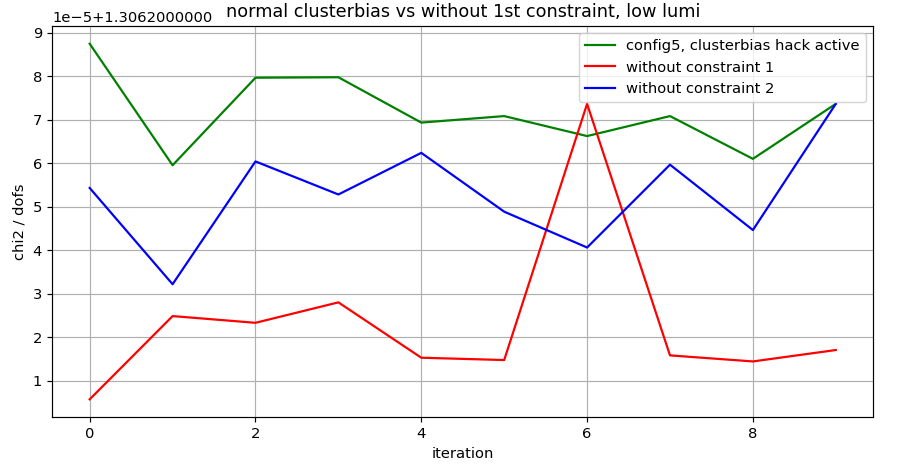
\includegraphics[width=0.8\textwidth]{plots/feb_6_2022/low_lumi_removed_constraints_vs_normal.png}
  \caption{impact of removing constraints from exisiting studies regarding chi2.}
  \label{fig:removeConst}
\end{figure}

We do want the least amount of constraints in the system so we also tested
the consequences of removing constraints from "config5".
The results are shown in figure \ref{fig:removeConst}.
The green curve shows the base configuration for comparison and in red the removal of the backlayer constraint in station 3 is shown. The blue curve shows the alignment results without the C-frame constraints.
The data samples used were from 2020 with the normal luminosity and an active clusterbias fix.
The selected track types are \textit{HighMomentumTTracks} for 10000 events.
On the one hand we see an improvement in $\chi^2 / \text{dof}$ when removing these constraints individually even if it is only on a very small scale of $\num{1e-5}$. On the
other hand we see that the $\chi^2 / \text{dof}$ after the last iteration is the same for the base config and for the blue measurement. The constraint removed in the red measurement seems to have the most impact from what was tested but the peak in iteration 6 has no logical
explanation. Additional analysis regarding constraint removal will be done in the future to analyse this phenomenon further.
Also the behavior of the not decreasing $\chi^2 / \text{dof}$ requires more testing.
What can be taken from this is that the removal of some constraints will help
the alignment but the cause of some abnormalities require more testing.

\section{Tests with input misalignments}
In order to evaluate the performance of the alignment with a given configuration in Monte Carlo simulations, input misalignments are used.

\chapter{Continuing Work}
\label{sec:continue}
For the remainder of the year commissioning of the SciFi will take place and instead of simulated data as used in this thesis, real data will be used. Using insights retrieved from the misalignment studies will help to estimate the alignment accuracy of the SciFi Tracker.

Input misalignments are a good way to retrieve information about how expected movements of the SciFi affect the alignment and monitoring outputs. When the data taking starts and and afterwards during times when the LHC is actively running, these simulated misalignment studies can be used for comparisons.
One sign of a good alignment is the absence of the layer splitting.
Similarly if the alignment is ``good'', in simulation it would converge towards the true aligned detector within three to five iterations.
If the convergence happens later there is either a bias hindering the alignment or there is a problem with the configuration itself.

After the work in this thesis there are still more open questions for the SciFi alignment. The cluster bias which prevents the alignment from working correctly is currently being analysed, and when this is fixed the alignment will require more testing with simulation and data. The plan is to repeat the studies presented in this thesis for the corrected simulation.

Additionally, there is another weak mode to consider in the SciFi, called the curvature bias.
\begin{figure}
    \centering
    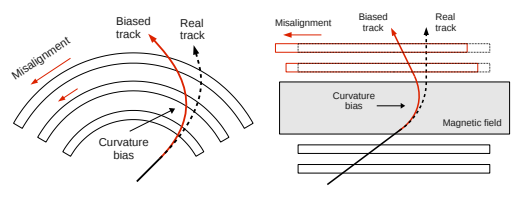
\includegraphics[width=0.8\textwidth]{plots/curvature_bias.png}
    \caption{Illustration of a curvature bias in a central detector (left) and a forward detector (right).}
    \label{fig:curvature}
\end{figure}
The curvature bias can appear in forward spectrometers with dipole magnets like the LHCb experiment and cylindrical detectors with solenoidal magnetic fields as shown in figure \ref{fig:curvature}.
In forward spectrometers like LHCb, the curvature bias can be caused by a superposition of relative shearing and rotation of the detectors surrounding the magnet. If a curvature bias is present, the reconstructed invariant mass of a two-body decay will be shifted proportionally to the momentum difference of the daughter particles in the final state\cite{1207.4756}.
There are different ways to control the curvature bias.
Performing alignments with the mentioned particle decays will be one approach to detect the curvature bias. In continuing studies particle alignment will be combined with shearing constraints. Plotting a known invariant mass distribution against the same distribution after the alignment could provide insights of the curvature bias because of the shift between them.
That is why alignment with particles will have an important role.
Another way to constrain the curvature bias is to use magnet-off data, but this only works if the detectors do not move when the magnetic field is turned on. Recent commissioning measurements of LHCb show that the SciFi detector does move when the magnet turns on.

In order to perform a successful alignment for the SciFi Tracker the detectors upstream of the SciFi need to be installed and aligned as well.
An essential part of the alignment is using correctly reconstructed long tracks, therefore the VELO has to be aligned to reconstruct good long tracks for the SciFi. 

\chapter{Future Work}
\label{sec:future}

Cluster bias analysis. particle alignment with misalignment tests.
Further analysis for weak modes.

% conclusion and outlook
\chapter{Conclusion}


\appendix
% Hier beginnt der Anhang, nummeriert in lateinischen Buchstaben
%\chapter{Ein Anhangskapitel}
Hier könnte ein Anhang stehen, falls Sie z.\,B.\ Code, Konstruktionszeichnungen oder Ähnliches mit in die Arbeit bringen wollen.
Im Normalfall stehen jedoch alle Ihre Resultate im Hauptteil der Bachelorarbeit und ein Anhang ist überflüssig.


\backmatter
\printbibliography
\chapter*{Danksagung}
An dieser Stelle m\"ochte ich mich bei all denen bedanken,
die mir w\"ahrend meiner Bachelorarbeit zur Seite standen und
ich mich immer unterst\"utzt haben.

Zuerst m\"ochte ich ich bei Herrn Professor Dr. Kevin Kr\"oninger
bedanken, durch welchen ich an seinem Lehrstuhl meine Bachelorarbeit
schreiben konnte. Au\ss erdem m\"ochte ich mich bei der Abteilung der
ATLAS Datenanalyse f\"ur die konstruktiven Anregungen bedanken.

Einen gro\ss en Dank spreche ich vor allem meinem Betreuer Dr.
Johannes Erdmann aus, der mich mit voller Unterst\"utzung und
wertvollen Ratschl\"agen und Hilfestellungen durch meine
Bachelorarbeit begleitet hat. Durch ihn habe ich viel
gelernt und bei Fragen konnte er mir stehts weiterhelfen.

Ich m\"ochte mich auch bei Herrn Professor Dr. Bernhard Spaan
f\"ur die Zweitkorrekur meiner Arbeit bedanken.

Mein Dank geb\"urt au\ss erdem Christopher Krause, Jan Lukas
Sp\"ah, Michael Windau, Sebastian L\"utge und Christian Beckmann
f\"ur die fachliche Kompetenz bei Fragen aller Art.

Zuletzt m\"ochte ich meiner Familie und Freunden daf\"ur danken,
dass sie mich w\"ahrend meines gesamten Studiums immer
unterst\"utzt und motiviert haben.

\cleardoublepage
\thispagestyle{empty}
% \section*{Eidesstattliche Versicherung}
% Ich versichere hiermit an Eides statt, dass ich die vorliegende Abschlussarbeit mit dem Titel \enquote{\thetitle} selbstständig und ohne unzulässige fremde Hilfe erbracht habe.
% Ich habe keine anderen als die angegebenen Quellen und Hilfsmittel benutzt, sowie wörtliche und sinngemäße Zitate kenntlich gemacht.
% Die Arbeit hat in gleicher oder ähnlicher Form noch keiner Prüfungsbehörde vorgelegen.
%
% \vspace*{1cm}\noindent
% \begin{center}
%   \begin{tabular}{@{}p{0.4\textwidth}@{\hspace{0.15\textwidth}}p{0.4\textwidth}@{}}
%   \rule{\linewidth}{0.25pt}& \rule{\linewidth}{0.25pt}\\
%   Ort, Datum & Unterschrift
%   \end{tabular}
% \end{center}
%
% \subsection*{Belehrung}
% Wer vorsätzlich gegen eine die Täuschung über Prüfungsleistungen betreffende Regelung einer Hochschulprüfungsordnung verstößt, handelt ordnungswidrig.
% Die Ordnungswidrigkeit kann mit einer Geldbuße von bis zu \SI[round-mode=places, round-precision=2]{50000}{€} geahndet werden.
% Zuständige Verwaltungsbehörde für die Verfolgung und Ahndung von Ordnungswidrigkeiten ist der Kanzler/die Kanzlerin der Technischen Universität Dortmund.
% Im Falle eines mehrfachen oder sonstigen schwerwiegenden Täuschungsversuches kann der Prüfling zudem exmatrikuliert werden \mbox{(\S\,63 Abs. 5 Hochschulgesetz --HG--).}
%
% Die Abgabe einer falschen Versicherung an Eides statt wird mit Freiheitsstrafe bis zu 3 Jahren oder mit Geldstrafe bestraft.
%
% Die Technische Universität Dortmund wird ggf.\ elektronische Vergleichswerkzeuge (wie z.\,B.\ die Software \enquote{turnitin}) zur Überprüfung von Ordnungswidrigkeiten in Prüfungsverfahren nutzen. \\[\baselineskip]
%
% \noindent Die oben stehende Belehrung habe ich zur Kenntnis genommen.\\[1cm]
% \begin{center}
% \begin{tabular}{@{}p{0.4\textwidth}@{\hspace{0.15\textwidth}}p{0.4\textwidth}@{}}
% \rule{\linewidth}{0.25pt}& \rule{\linewidth}{0.25pt}\\
% Ort, Datum & Unterschrift
% \end{tabular}
% \end{center}

\begin{figure}
  \centering
  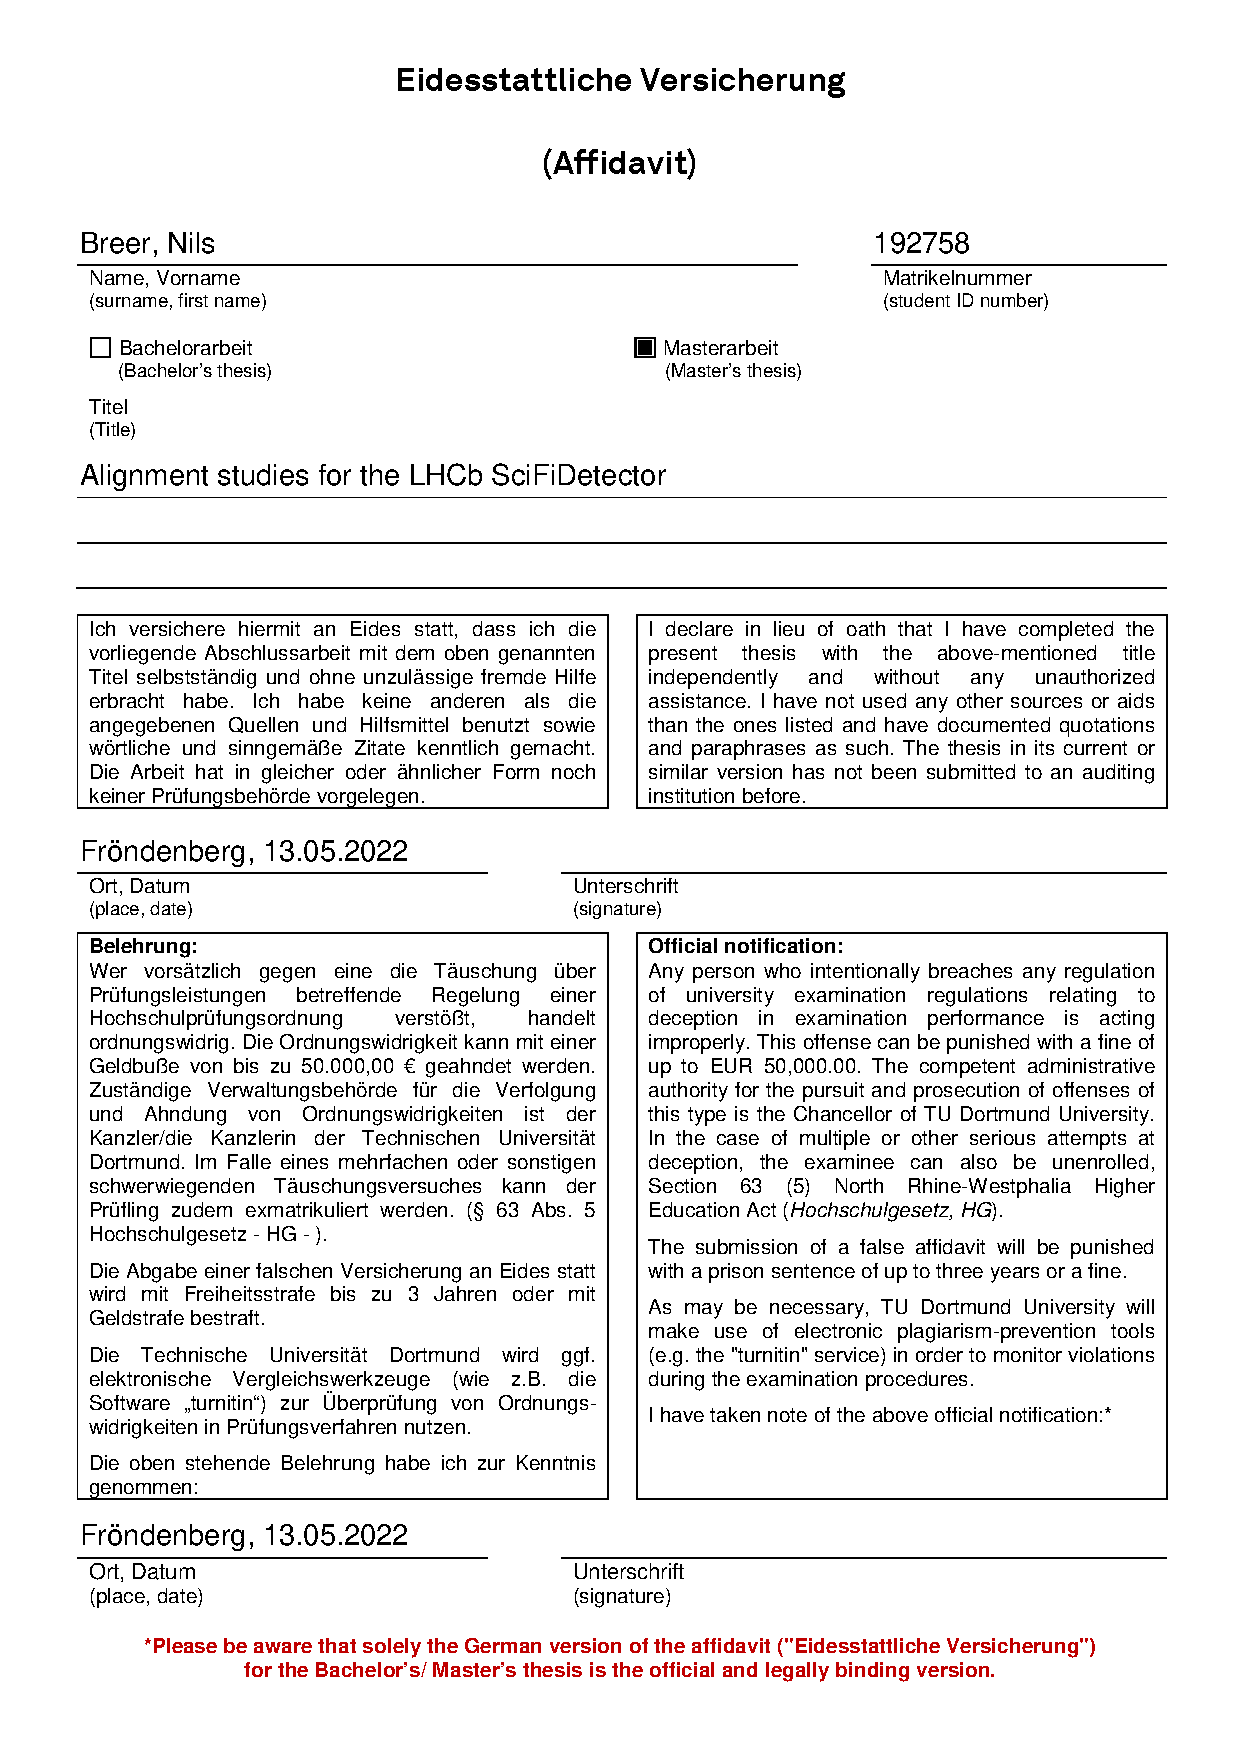
\includegraphics[width=\textwidth]{Eidesstattliche_Versicherung.pdf}
\end{figure}

\end{document}
